% =============================================================================
% InstructorHandouts/CS401/02-number-systems-arithmetic-instructor-handout.tex
% Instructor Handout 2: Number Systems, Representation, and Arithmetic Hardware
%
% INSTRUCTOR-ONLY. Complete, self-contained teaching guide -- explanation,
% embedded diagrams, presentation guidance, and delivery commentary are woven
% together per topic (not split into separate documents/sections), so an
% instructor can teach directly from this file with no slides or Notes open.
% Explanations/diagrams/examples trace to Slides/CS401/02-number-systems-arithmetic.tex
% and Notes/CS401/02-number-systems-arithmetic-notes.tex; "Teaching note"
% asides are instructor judgment, visually distinguished but not a separate
% section.
%
% Anchor readings: Hamacher, Computer Organization, Ch. 2 (chapter-level, not
%   indexed); Mano, Computer System Architecture, Ch. 1 (chapter-level, not
%   indexed); Patterson & Hennessy, Computer Organization and Design, ARM
%   Edition, Sec. 3.2 (p.188), Sec. 3.3 (p.191), Sec. 3.4 (p.197) -- page-cited
%   (PattersonHennessy2017 index built 2026-08-07).
%
% Compile with: cd InstructorHandouts/CS401 &&
%   TEXINPUTS=../../Preambles;$TEXINPUTS xelatex -interaction=nonstopmode 02-number-systems-arithmetic-instructor-handout.tex
% =============================================================================

\documentclass[11pt]{article}
\usepackage[margin=1in]{geometry}
% =============================================================================
% Preambles/header.tex — shared LaTeX/Beamer preamble for this project
%
% Use from a Beamer lecture by prepending:
%     % =============================================================================
% Preambles/header.tex — shared LaTeX/Beamer preamble for this project
%
% Use from a Beamer lecture by prepending:
%     % =============================================================================
% Preambles/header.tex — shared LaTeX/Beamer preamble for this project
%
% Use from a Beamer lecture by prepending:
%     \input{header}
% and compiling with TEXINPUTS=../Preambles:$TEXINPUTS (the /compile-latex
% skill does this automatically).
%
% PALETTE CONTRACT. Color names defined here MUST match the names in
% Quarto/theme-template.scss so Beamer and Quarto renderings use the same
% palette. The scripts/check-palette-sync.sh script enforces this.
%
% To customize: edit the HEX values below AND the matching $variable in
% Quarto/theme-template.scss, then run scripts/check-palette-sync.sh.
%
% TITLE PAGE. A formal, serif (Libertine) title-page template is defined in
% the Beamer-only block below (\setbeamertemplate{title page}) -- title,
% subtitle, a thin gold rule, then \author/\institute/\date. Frametitle and
% body text remain on Beamer's sans-serif default. No SCSS counterpart is
% needed for this (font/layout only, no new colors).
% =============================================================================

% -----------------------------------------------------------------------------
% Engine detection + encoding
%
% Our /compile-latex skill uses XeLaTeX, where inputenc is unnecessary and
% can produce encoding warnings. Only load inputenc under pdfTeX.
% -----------------------------------------------------------------------------
\usepackage{iftex}
\ifPDFTeX
  \usepackage[utf8]{inputenc}
\fi

\usepackage{amsmath, amssymb, amsthm}
\usepackage{booktabs}
\usepackage{graphicx}

% -----------------------------------------------------------------------------
% Serif face for the title page (formal/academic look). Linux Libertine is
% XeLaTeX- and pdfTeX-safe and redefines \rmdefault, so \rmfamily picks it up
% everywhere \rmfamily is used explicitly. Body text and frametitles stay on
% Beamer's own sans-serif default (unaffected) -- only the title-page
% \setbeamerfont{...} overrides below opt in to \rmfamily.
% -----------------------------------------------------------------------------
\usepackage{libertine}

% -----------------------------------------------------------------------------
% PALETTE — mirrors Quarto/theme-template.scss variable names.
% Load xcolor and define colors BEFORE anything that references them
% (notably hyperref, hypersetup, and the Beamer color assignments).
% -----------------------------------------------------------------------------
\usepackage{xcolor}

\definecolor{primary-blue}{HTML}{012169}      % headings, accents
\definecolor{primary-gold}{HTML}{B9975B}      % emphasis, borders
\definecolor{highlight-yellow}{HTML}{F2A900}  % markers, alerts
\definecolor{light-bg}{HTML}{E8EDF5}          % title / section backgrounds
\definecolor{jet}{HTML}{1A1A1A}               % body text

% Semantic colors (used in diagrams and annotations)
\definecolor{positive}{HTML}{15803D}          % good / observed / identified
\definecolor{negative}{HTML}{B91C1C}          % bad / problematic / bias
\definecolor{neutral}{HTML}{525252}           % reference / context

% Highlight accents (match .hi-* classes in the SCSS)
\definecolor{hi-slate}{HTML}{314F4F}
\definecolor{hi-green}{HTML}{2E8B57}
\definecolor{hi-red}{HTML}{C41E3A}

% Semantic aliases so skill templates and snippets can write
% \textcolor{accent}{...} without hard-coding "primary-blue".
\colorlet{accent}{primary-blue}
\colorlet{accent2}{primary-gold}

% -----------------------------------------------------------------------------
% Hyperref — loaded AFTER xcolor + palette so link colors resolve.
% -----------------------------------------------------------------------------
\usepackage{hyperref}
\hypersetup{colorlinks=true, linkcolor=primary-blue, urlcolor=primary-blue,
            citecolor=primary-blue, pdfborder={0 0 0}}

% -----------------------------------------------------------------------------
% Course code — set once per deck (after \input{header}, before \begin{document})
% via \coursecode{CS401}. Shown in the footer on every slide so a deck's course
% is identifiable without opening the title page. Empty by default.
% -----------------------------------------------------------------------------
\makeatletter
\newcommand{\coursecode}[1]{\gdef\@coursecodetext{#1}}
\gdef\@coursecodetext{}
\makeatother

% -----------------------------------------------------------------------------
% Beamer theme assignments (only apply under Beamer).
%
% We detect Beamer via \@ifclassloaded{beamer}, which is the documented,
% non-internal way. This must be wrapped in \makeatletter/\makeatother
% because \@ifclassloaded contains an @-catcode character.
% -----------------------------------------------------------------------------
\makeatletter
\@ifclassloaded{beamer}{%
  \usefonttheme{professionalfonts}
  \setbeamercolor{structure}{fg=primary-blue}
  \setbeamercolor{frametitle}{fg=primary-blue}
  \setbeamercolor{title}{fg=primary-blue}
  \setbeamercolor{subtitle}{fg=primary-gold}
  \setbeamercolor{author}{fg=primary-blue}
  \setbeamercolor{institute}{fg=neutral}
  \setbeamercolor{date}{fg=primary-gold}
  \setbeamercolor{itemize item}{fg=primary-blue}
  \setbeamercolor{itemize subitem}{fg=primary-gold}
  \setbeamercolor{alerted text}{fg=primary-gold}
  \setbeamercolor{block title}{fg=white, bg=primary-blue}
  \setbeamercolor{block body}{bg=light-bg}
  % Semantic block variants: block=definition/concept (blue), exampleblock=
  % worked example (green/positive), alertblock=key takeaway or caution (gold).
  % Keep to <=2 colored boxes per slide across ALL three variants (INV-7).
  \setbeamercolor{block title example}{fg=white, bg=positive}
  \setbeamercolor{block body example}{bg=light-bg}
  \setbeamercolor{block title alerted}{fg=white, bg=primary-gold}
  \setbeamercolor{block body alerted}{bg=light-bg}

  % ---------------------------------------------------------------------------
  % Formal title page: serif (Libertine, via \rmfamily) for title-page
  % elements only. Body text, itemize, and frametitle are intentionally left
  % on Beamer's sans-serif default -- \usebeamerfont{title} is also what
  % \transitionslide (below) uses for its big centered text, so section
  % transitions pick up the same serif treatment for free.
  % ---------------------------------------------------------------------------
  \setbeamerfont{title}{family=\rmfamily, series=\bfseries, size=\Large}
  \setbeamerfont{subtitle}{family=\rmfamily, shape=\itshape, size=\normalsize}
  \setbeamerfont{author}{family=\rmfamily, size=\normalsize}
  \setbeamerfont{institute}{family=\rmfamily, size=\scriptsize}
  \setbeamerfont{date}{family=\rmfamily, size=\scriptsize}

  \setbeamertemplate{title page}{
    \vfill
    \begin{center}
      {\usebeamerfont{title}\usebeamercolor[fg]{title}\inserttitle\par}
      \vspace{0.15cm}
      {\usebeamerfont{subtitle}\usebeamercolor[fg]{subtitle}\insertsubtitle\par}
      \vspace{0.45cm}
      {\color{primary-gold}\rule{0.42\textwidth}{0.6pt}\par}
      \vspace{0.45cm}
      {\usebeamerfont{author}\usebeamercolor[fg]{author}\insertauthor\par}
      \vspace{0.35cm}
      {\usebeamerfont{institute}\usebeamercolor[fg]{institute}\insertinstitute\par}
      \vspace{0.35cm}
      {\usebeamerfont{date}\usebeamercolor[fg]{date}\insertdate\par}
    \end{center}
    \vfill
  }

  % Minimal footer: course code (left) + page X / N (right), no navigation clutter
  \setbeamertemplate{navigation symbols}{}
  \setbeamertemplate{footline}{%
    \color{neutral}\footnotesize\hspace{0.7em}\@coursecodetext\hfill
    \insertframenumber/\inserttotalframenumber\hspace{0.7em}\vspace{0.3em}}
}{}
\makeatother

% -----------------------------------------------------------------------------
% TikZ setup — libraries the snippet gallery uses
% -----------------------------------------------------------------------------
\usepackage{tikz}
\usetikzlibrary{arrows.meta, positioning, calc, decorations.pathreplacing,
                fit, shapes.geometric, backgrounds}

% Shared TikZ styles — snippets and hand-written diagrams can pick these up
% via `\begin{tikzpicture}[every node/.style={...}]` or by naming specific
% styles (e.g., `\node[dag-node] (X) at (0,0) {X};`).
\tikzset{
  % Node styles for causal DAGs and similar
  dag-node/.style = {
    draw=primary-blue, fill=light-bg, rounded corners=2pt,
    minimum width=1.2cm, minimum height=0.9cm, align=center, font=\small
  },
  decision-node/.style = {
    draw=primary-gold, fill=white, diamond, aspect=1.8,
    minimum width=1.8cm, minimum height=1.2cm, align=center, font=\small,
    inner sep=1pt
  },
  % Edge styles — observed vs counterfactual
  observed-edge/.style = {-{Latex[length=2.5mm]}, thick, draw=jet},
  counterfactual-edge/.style = {-{Latex[length=2.5mm]}, thick, draw=neutral, dashed},
  confound-edge/.style = {-{Latex[length=2.5mm]}, thick, draw=negative, dashed},
  % Data-point styles for plots
  observed-dot/.style = {fill=primary-blue, draw=primary-blue, circle, inner sep=1.2pt},
  counterfactual-dot/.style = {fill=white, draw=neutral, circle, inner sep=1.2pt}
}

% -----------------------------------------------------------------------------
% Convenience macros
% -----------------------------------------------------------------------------
\newcommand{\muted}[1]{\textcolor{neutral}{#1}}
\newcommand{\key}[1]{\textcolor{primary-gold}{\textbf{#1}}}
\newcommand{\good}[1]{\textcolor{positive}{#1}}
\newcommand{\bad}[1]{\textcolor{negative}{#1}}

% Standout frame macro: full-bleed dark background for section transitions.
% Beamer-only (uses \begin{frame}/\setbeamercolor/\usebeamerfont) -- do not
% call from an article-class file (e.g. Notes/<CODE>/*-notes.tex). \muted,
% \key, \good, \bad, and \coursecode above are plain xcolor/gdef and are
% safe to use from either class; verified when Notes/article-class support
% was added.
% Expand: \transitionslide{Your transition title}
\newcommand{\transitionslide}[1]{%
  \begingroup
  \setbeamercolor{background canvas}{bg=primary-blue}
  \begin{frame}[plain]
    \centering
    \vfill
    {\usebeamerfont{title}\color{white}\Large #1\par}
    \vfill
  \end{frame}
  \endgroup
}

% and compiling with TEXINPUTS=../Preambles:$TEXINPUTS (the /compile-latex
% skill does this automatically).
%
% PALETTE CONTRACT. Color names defined here MUST match the names in
% Quarto/theme-template.scss so Beamer and Quarto renderings use the same
% palette. The scripts/check-palette-sync.sh script enforces this.
%
% To customize: edit the HEX values below AND the matching $variable in
% Quarto/theme-template.scss, then run scripts/check-palette-sync.sh.
%
% TITLE PAGE. A formal, serif (Libertine) title-page template is defined in
% the Beamer-only block below (\setbeamertemplate{title page}) -- title,
% subtitle, a thin gold rule, then \author/\institute/\date. Frametitle and
% body text remain on Beamer's sans-serif default. No SCSS counterpart is
% needed for this (font/layout only, no new colors).
% =============================================================================

% -----------------------------------------------------------------------------
% Engine detection + encoding
%
% Our /compile-latex skill uses XeLaTeX, where inputenc is unnecessary and
% can produce encoding warnings. Only load inputenc under pdfTeX.
% -----------------------------------------------------------------------------
\usepackage{iftex}
\ifPDFTeX
  \usepackage[utf8]{inputenc}
\fi

\usepackage{amsmath, amssymb, amsthm}
\usepackage{booktabs}
\usepackage{graphicx}

% -----------------------------------------------------------------------------
% Serif face for the title page (formal/academic look). Linux Libertine is
% XeLaTeX- and pdfTeX-safe and redefines \rmdefault, so \rmfamily picks it up
% everywhere \rmfamily is used explicitly. Body text and frametitles stay on
% Beamer's own sans-serif default (unaffected) -- only the title-page
% \setbeamerfont{...} overrides below opt in to \rmfamily.
% -----------------------------------------------------------------------------
\usepackage{libertine}

% -----------------------------------------------------------------------------
% PALETTE — mirrors Quarto/theme-template.scss variable names.
% Load xcolor and define colors BEFORE anything that references them
% (notably hyperref, hypersetup, and the Beamer color assignments).
% -----------------------------------------------------------------------------
\usepackage{xcolor}

\definecolor{primary-blue}{HTML}{012169}      % headings, accents
\definecolor{primary-gold}{HTML}{B9975B}      % emphasis, borders
\definecolor{highlight-yellow}{HTML}{F2A900}  % markers, alerts
\definecolor{light-bg}{HTML}{E8EDF5}          % title / section backgrounds
\definecolor{jet}{HTML}{1A1A1A}               % body text

% Semantic colors (used in diagrams and annotations)
\definecolor{positive}{HTML}{15803D}          % good / observed / identified
\definecolor{negative}{HTML}{B91C1C}          % bad / problematic / bias
\definecolor{neutral}{HTML}{525252}           % reference / context

% Highlight accents (match .hi-* classes in the SCSS)
\definecolor{hi-slate}{HTML}{314F4F}
\definecolor{hi-green}{HTML}{2E8B57}
\definecolor{hi-red}{HTML}{C41E3A}

% Semantic aliases so skill templates and snippets can write
% \textcolor{accent}{...} without hard-coding "primary-blue".
\colorlet{accent}{primary-blue}
\colorlet{accent2}{primary-gold}

% -----------------------------------------------------------------------------
% Hyperref — loaded AFTER xcolor + palette so link colors resolve.
% -----------------------------------------------------------------------------
\usepackage{hyperref}
\hypersetup{colorlinks=true, linkcolor=primary-blue, urlcolor=primary-blue,
            citecolor=primary-blue, pdfborder={0 0 0}}

% -----------------------------------------------------------------------------
% Course code — set once per deck (after % =============================================================================
% Preambles/header.tex — shared LaTeX/Beamer preamble for this project
%
% Use from a Beamer lecture by prepending:
%     \input{header}
% and compiling with TEXINPUTS=../Preambles:$TEXINPUTS (the /compile-latex
% skill does this automatically).
%
% PALETTE CONTRACT. Color names defined here MUST match the names in
% Quarto/theme-template.scss so Beamer and Quarto renderings use the same
% palette. The scripts/check-palette-sync.sh script enforces this.
%
% To customize: edit the HEX values below AND the matching $variable in
% Quarto/theme-template.scss, then run scripts/check-palette-sync.sh.
%
% TITLE PAGE. A formal, serif (Libertine) title-page template is defined in
% the Beamer-only block below (\setbeamertemplate{title page}) -- title,
% subtitle, a thin gold rule, then \author/\institute/\date. Frametitle and
% body text remain on Beamer's sans-serif default. No SCSS counterpart is
% needed for this (font/layout only, no new colors).
% =============================================================================

% -----------------------------------------------------------------------------
% Engine detection + encoding
%
% Our /compile-latex skill uses XeLaTeX, where inputenc is unnecessary and
% can produce encoding warnings. Only load inputenc under pdfTeX.
% -----------------------------------------------------------------------------
\usepackage{iftex}
\ifPDFTeX
  \usepackage[utf8]{inputenc}
\fi

\usepackage{amsmath, amssymb, amsthm}
\usepackage{booktabs}
\usepackage{graphicx}

% -----------------------------------------------------------------------------
% Serif face for the title page (formal/academic look). Linux Libertine is
% XeLaTeX- and pdfTeX-safe and redefines \rmdefault, so \rmfamily picks it up
% everywhere \rmfamily is used explicitly. Body text and frametitles stay on
% Beamer's own sans-serif default (unaffected) -- only the title-page
% \setbeamerfont{...} overrides below opt in to \rmfamily.
% -----------------------------------------------------------------------------
\usepackage{libertine}

% -----------------------------------------------------------------------------
% PALETTE — mirrors Quarto/theme-template.scss variable names.
% Load xcolor and define colors BEFORE anything that references them
% (notably hyperref, hypersetup, and the Beamer color assignments).
% -----------------------------------------------------------------------------
\usepackage{xcolor}

\definecolor{primary-blue}{HTML}{012169}      % headings, accents
\definecolor{primary-gold}{HTML}{B9975B}      % emphasis, borders
\definecolor{highlight-yellow}{HTML}{F2A900}  % markers, alerts
\definecolor{light-bg}{HTML}{E8EDF5}          % title / section backgrounds
\definecolor{jet}{HTML}{1A1A1A}               % body text

% Semantic colors (used in diagrams and annotations)
\definecolor{positive}{HTML}{15803D}          % good / observed / identified
\definecolor{negative}{HTML}{B91C1C}          % bad / problematic / bias
\definecolor{neutral}{HTML}{525252}           % reference / context

% Highlight accents (match .hi-* classes in the SCSS)
\definecolor{hi-slate}{HTML}{314F4F}
\definecolor{hi-green}{HTML}{2E8B57}
\definecolor{hi-red}{HTML}{C41E3A}

% Semantic aliases so skill templates and snippets can write
% \textcolor{accent}{...} without hard-coding "primary-blue".
\colorlet{accent}{primary-blue}
\colorlet{accent2}{primary-gold}

% -----------------------------------------------------------------------------
% Hyperref — loaded AFTER xcolor + palette so link colors resolve.
% -----------------------------------------------------------------------------
\usepackage{hyperref}
\hypersetup{colorlinks=true, linkcolor=primary-blue, urlcolor=primary-blue,
            citecolor=primary-blue, pdfborder={0 0 0}}

% -----------------------------------------------------------------------------
% Course code — set once per deck (after \input{header}, before \begin{document})
% via \coursecode{CS401}. Shown in the footer on every slide so a deck's course
% is identifiable without opening the title page. Empty by default.
% -----------------------------------------------------------------------------
\makeatletter
\newcommand{\coursecode}[1]{\gdef\@coursecodetext{#1}}
\gdef\@coursecodetext{}
\makeatother

% -----------------------------------------------------------------------------
% Beamer theme assignments (only apply under Beamer).
%
% We detect Beamer via \@ifclassloaded{beamer}, which is the documented,
% non-internal way. This must be wrapped in \makeatletter/\makeatother
% because \@ifclassloaded contains an @-catcode character.
% -----------------------------------------------------------------------------
\makeatletter
\@ifclassloaded{beamer}{%
  \usefonttheme{professionalfonts}
  \setbeamercolor{structure}{fg=primary-blue}
  \setbeamercolor{frametitle}{fg=primary-blue}
  \setbeamercolor{title}{fg=primary-blue}
  \setbeamercolor{subtitle}{fg=primary-gold}
  \setbeamercolor{author}{fg=primary-blue}
  \setbeamercolor{institute}{fg=neutral}
  \setbeamercolor{date}{fg=primary-gold}
  \setbeamercolor{itemize item}{fg=primary-blue}
  \setbeamercolor{itemize subitem}{fg=primary-gold}
  \setbeamercolor{alerted text}{fg=primary-gold}
  \setbeamercolor{block title}{fg=white, bg=primary-blue}
  \setbeamercolor{block body}{bg=light-bg}
  % Semantic block variants: block=definition/concept (blue), exampleblock=
  % worked example (green/positive), alertblock=key takeaway or caution (gold).
  % Keep to <=2 colored boxes per slide across ALL three variants (INV-7).
  \setbeamercolor{block title example}{fg=white, bg=positive}
  \setbeamercolor{block body example}{bg=light-bg}
  \setbeamercolor{block title alerted}{fg=white, bg=primary-gold}
  \setbeamercolor{block body alerted}{bg=light-bg}

  % ---------------------------------------------------------------------------
  % Formal title page: serif (Libertine, via \rmfamily) for title-page
  % elements only. Body text, itemize, and frametitle are intentionally left
  % on Beamer's sans-serif default -- \usebeamerfont{title} is also what
  % \transitionslide (below) uses for its big centered text, so section
  % transitions pick up the same serif treatment for free.
  % ---------------------------------------------------------------------------
  \setbeamerfont{title}{family=\rmfamily, series=\bfseries, size=\Large}
  \setbeamerfont{subtitle}{family=\rmfamily, shape=\itshape, size=\normalsize}
  \setbeamerfont{author}{family=\rmfamily, size=\normalsize}
  \setbeamerfont{institute}{family=\rmfamily, size=\scriptsize}
  \setbeamerfont{date}{family=\rmfamily, size=\scriptsize}

  \setbeamertemplate{title page}{
    \vfill
    \begin{center}
      {\usebeamerfont{title}\usebeamercolor[fg]{title}\inserttitle\par}
      \vspace{0.15cm}
      {\usebeamerfont{subtitle}\usebeamercolor[fg]{subtitle}\insertsubtitle\par}
      \vspace{0.45cm}
      {\color{primary-gold}\rule{0.42\textwidth}{0.6pt}\par}
      \vspace{0.45cm}
      {\usebeamerfont{author}\usebeamercolor[fg]{author}\insertauthor\par}
      \vspace{0.35cm}
      {\usebeamerfont{institute}\usebeamercolor[fg]{institute}\insertinstitute\par}
      \vspace{0.35cm}
      {\usebeamerfont{date}\usebeamercolor[fg]{date}\insertdate\par}
    \end{center}
    \vfill
  }

  % Minimal footer: course code (left) + page X / N (right), no navigation clutter
  \setbeamertemplate{navigation symbols}{}
  \setbeamertemplate{footline}{%
    \color{neutral}\footnotesize\hspace{0.7em}\@coursecodetext\hfill
    \insertframenumber/\inserttotalframenumber\hspace{0.7em}\vspace{0.3em}}
}{}
\makeatother

% -----------------------------------------------------------------------------
% TikZ setup — libraries the snippet gallery uses
% -----------------------------------------------------------------------------
\usepackage{tikz}
\usetikzlibrary{arrows.meta, positioning, calc, decorations.pathreplacing,
                fit, shapes.geometric, backgrounds}

% Shared TikZ styles — snippets and hand-written diagrams can pick these up
% via `\begin{tikzpicture}[every node/.style={...}]` or by naming specific
% styles (e.g., `\node[dag-node] (X) at (0,0) {X};`).
\tikzset{
  % Node styles for causal DAGs and similar
  dag-node/.style = {
    draw=primary-blue, fill=light-bg, rounded corners=2pt,
    minimum width=1.2cm, minimum height=0.9cm, align=center, font=\small
  },
  decision-node/.style = {
    draw=primary-gold, fill=white, diamond, aspect=1.8,
    minimum width=1.8cm, minimum height=1.2cm, align=center, font=\small,
    inner sep=1pt
  },
  % Edge styles — observed vs counterfactual
  observed-edge/.style = {-{Latex[length=2.5mm]}, thick, draw=jet},
  counterfactual-edge/.style = {-{Latex[length=2.5mm]}, thick, draw=neutral, dashed},
  confound-edge/.style = {-{Latex[length=2.5mm]}, thick, draw=negative, dashed},
  % Data-point styles for plots
  observed-dot/.style = {fill=primary-blue, draw=primary-blue, circle, inner sep=1.2pt},
  counterfactual-dot/.style = {fill=white, draw=neutral, circle, inner sep=1.2pt}
}

% -----------------------------------------------------------------------------
% Convenience macros
% -----------------------------------------------------------------------------
\newcommand{\muted}[1]{\textcolor{neutral}{#1}}
\newcommand{\key}[1]{\textcolor{primary-gold}{\textbf{#1}}}
\newcommand{\good}[1]{\textcolor{positive}{#1}}
\newcommand{\bad}[1]{\textcolor{negative}{#1}}

% Standout frame macro: full-bleed dark background for section transitions.
% Beamer-only (uses \begin{frame}/\setbeamercolor/\usebeamerfont) -- do not
% call from an article-class file (e.g. Notes/<CODE>/*-notes.tex). \muted,
% \key, \good, \bad, and \coursecode above are plain xcolor/gdef and are
% safe to use from either class; verified when Notes/article-class support
% was added.
% Expand: \transitionslide{Your transition title}
\newcommand{\transitionslide}[1]{%
  \begingroup
  \setbeamercolor{background canvas}{bg=primary-blue}
  \begin{frame}[plain]
    \centering
    \vfill
    {\usebeamerfont{title}\color{white}\Large #1\par}
    \vfill
  \end{frame}
  \endgroup
}
, before \begin{document})
% via \coursecode{CS401}. Shown in the footer on every slide so a deck's course
% is identifiable without opening the title page. Empty by default.
% -----------------------------------------------------------------------------
\makeatletter
\newcommand{\coursecode}[1]{\gdef\@coursecodetext{#1}}
\gdef\@coursecodetext{}
\makeatother

% -----------------------------------------------------------------------------
% Beamer theme assignments (only apply under Beamer).
%
% We detect Beamer via \@ifclassloaded{beamer}, which is the documented,
% non-internal way. This must be wrapped in \makeatletter/\makeatother
% because \@ifclassloaded contains an @-catcode character.
% -----------------------------------------------------------------------------
\makeatletter
\@ifclassloaded{beamer}{%
  \usefonttheme{professionalfonts}
  \setbeamercolor{structure}{fg=primary-blue}
  \setbeamercolor{frametitle}{fg=primary-blue}
  \setbeamercolor{title}{fg=primary-blue}
  \setbeamercolor{subtitle}{fg=primary-gold}
  \setbeamercolor{author}{fg=primary-blue}
  \setbeamercolor{institute}{fg=neutral}
  \setbeamercolor{date}{fg=primary-gold}
  \setbeamercolor{itemize item}{fg=primary-blue}
  \setbeamercolor{itemize subitem}{fg=primary-gold}
  \setbeamercolor{alerted text}{fg=primary-gold}
  \setbeamercolor{block title}{fg=white, bg=primary-blue}
  \setbeamercolor{block body}{bg=light-bg}
  % Semantic block variants: block=definition/concept (blue), exampleblock=
  % worked example (green/positive), alertblock=key takeaway or caution (gold).
  % Keep to <=2 colored boxes per slide across ALL three variants (INV-7).
  \setbeamercolor{block title example}{fg=white, bg=positive}
  \setbeamercolor{block body example}{bg=light-bg}
  \setbeamercolor{block title alerted}{fg=white, bg=primary-gold}
  \setbeamercolor{block body alerted}{bg=light-bg}

  % ---------------------------------------------------------------------------
  % Formal title page: serif (Libertine, via \rmfamily) for title-page
  % elements only. Body text, itemize, and frametitle are intentionally left
  % on Beamer's sans-serif default -- \usebeamerfont{title} is also what
  % \transitionslide (below) uses for its big centered text, so section
  % transitions pick up the same serif treatment for free.
  % ---------------------------------------------------------------------------
  \setbeamerfont{title}{family=\rmfamily, series=\bfseries, size=\Large}
  \setbeamerfont{subtitle}{family=\rmfamily, shape=\itshape, size=\normalsize}
  \setbeamerfont{author}{family=\rmfamily, size=\normalsize}
  \setbeamerfont{institute}{family=\rmfamily, size=\scriptsize}
  \setbeamerfont{date}{family=\rmfamily, size=\scriptsize}

  \setbeamertemplate{title page}{
    \vfill
    \begin{center}
      {\usebeamerfont{title}\usebeamercolor[fg]{title}\inserttitle\par}
      \vspace{0.15cm}
      {\usebeamerfont{subtitle}\usebeamercolor[fg]{subtitle}\insertsubtitle\par}
      \vspace{0.45cm}
      {\color{primary-gold}\rule{0.42\textwidth}{0.6pt}\par}
      \vspace{0.45cm}
      {\usebeamerfont{author}\usebeamercolor[fg]{author}\insertauthor\par}
      \vspace{0.35cm}
      {\usebeamerfont{institute}\usebeamercolor[fg]{institute}\insertinstitute\par}
      \vspace{0.35cm}
      {\usebeamerfont{date}\usebeamercolor[fg]{date}\insertdate\par}
    \end{center}
    \vfill
  }

  % Minimal footer: course code (left) + page X / N (right), no navigation clutter
  \setbeamertemplate{navigation symbols}{}
  \setbeamertemplate{footline}{%
    \color{neutral}\footnotesize\hspace{0.7em}\@coursecodetext\hfill
    \insertframenumber/\inserttotalframenumber\hspace{0.7em}\vspace{0.3em}}
}{}
\makeatother

% -----------------------------------------------------------------------------
% TikZ setup — libraries the snippet gallery uses
% -----------------------------------------------------------------------------
\usepackage{tikz}
\usetikzlibrary{arrows.meta, positioning, calc, decorations.pathreplacing,
                fit, shapes.geometric, backgrounds}

% Shared TikZ styles — snippets and hand-written diagrams can pick these up
% via `\begin{tikzpicture}[every node/.style={...}]` or by naming specific
% styles (e.g., `\node[dag-node] (X) at (0,0) {X};`).
\tikzset{
  % Node styles for causal DAGs and similar
  dag-node/.style = {
    draw=primary-blue, fill=light-bg, rounded corners=2pt,
    minimum width=1.2cm, minimum height=0.9cm, align=center, font=\small
  },
  decision-node/.style = {
    draw=primary-gold, fill=white, diamond, aspect=1.8,
    minimum width=1.8cm, minimum height=1.2cm, align=center, font=\small,
    inner sep=1pt
  },
  % Edge styles — observed vs counterfactual
  observed-edge/.style = {-{Latex[length=2.5mm]}, thick, draw=jet},
  counterfactual-edge/.style = {-{Latex[length=2.5mm]}, thick, draw=neutral, dashed},
  confound-edge/.style = {-{Latex[length=2.5mm]}, thick, draw=negative, dashed},
  % Data-point styles for plots
  observed-dot/.style = {fill=primary-blue, draw=primary-blue, circle, inner sep=1.2pt},
  counterfactual-dot/.style = {fill=white, draw=neutral, circle, inner sep=1.2pt}
}

% -----------------------------------------------------------------------------
% Convenience macros
% -----------------------------------------------------------------------------
\newcommand{\muted}[1]{\textcolor{neutral}{#1}}
\newcommand{\key}[1]{\textcolor{primary-gold}{\textbf{#1}}}
\newcommand{\good}[1]{\textcolor{positive}{#1}}
\newcommand{\bad}[1]{\textcolor{negative}{#1}}

% Standout frame macro: full-bleed dark background for section transitions.
% Beamer-only (uses \begin{frame}/\setbeamercolor/\usebeamerfont) -- do not
% call from an article-class file (e.g. Notes/<CODE>/*-notes.tex). \muted,
% \key, \good, \bad, and \coursecode above are plain xcolor/gdef and are
% safe to use from either class; verified when Notes/article-class support
% was added.
% Expand: \transitionslide{Your transition title}
\newcommand{\transitionslide}[1]{%
  \begingroup
  \setbeamercolor{background canvas}{bg=primary-blue}
  \begin{frame}[plain]
    \centering
    \vfill
    {\usebeamerfont{title}\color{white}\Large #1\par}
    \vfill
  \end{frame}
  \endgroup
}

% and compiling with TEXINPUTS=../Preambles:$TEXINPUTS (the /compile-latex
% skill does this automatically).
%
% PALETTE CONTRACT. Color names defined here MUST match the names in
% Quarto/theme-template.scss so Beamer and Quarto renderings use the same
% palette. The scripts/check-palette-sync.sh script enforces this.
%
% To customize: edit the HEX values below AND the matching $variable in
% Quarto/theme-template.scss, then run scripts/check-palette-sync.sh.
%
% TITLE PAGE. A formal, serif (Libertine) title-page template is defined in
% the Beamer-only block below (\setbeamertemplate{title page}) -- title,
% subtitle, a thin gold rule, then \author/\institute/\date. Frametitle and
% body text remain on Beamer's sans-serif default. No SCSS counterpart is
% needed for this (font/layout only, no new colors).
% =============================================================================

% -----------------------------------------------------------------------------
% Engine detection + encoding
%
% Our /compile-latex skill uses XeLaTeX, where inputenc is unnecessary and
% can produce encoding warnings. Only load inputenc under pdfTeX.
% -----------------------------------------------------------------------------
\usepackage{iftex}
\ifPDFTeX
  \usepackage[utf8]{inputenc}
\fi

\usepackage{amsmath, amssymb, amsthm}
\usepackage{booktabs}
\usepackage{graphicx}

% -----------------------------------------------------------------------------
% Serif face for the title page (formal/academic look). Linux Libertine is
% XeLaTeX- and pdfTeX-safe and redefines \rmdefault, so \rmfamily picks it up
% everywhere \rmfamily is used explicitly. Body text and frametitles stay on
% Beamer's own sans-serif default (unaffected) -- only the title-page
% \setbeamerfont{...} overrides below opt in to \rmfamily.
% -----------------------------------------------------------------------------
\usepackage{libertine}

% -----------------------------------------------------------------------------
% PALETTE — mirrors Quarto/theme-template.scss variable names.
% Load xcolor and define colors BEFORE anything that references them
% (notably hyperref, hypersetup, and the Beamer color assignments).
% -----------------------------------------------------------------------------
\usepackage{xcolor}

\definecolor{primary-blue}{HTML}{012169}      % headings, accents
\definecolor{primary-gold}{HTML}{B9975B}      % emphasis, borders
\definecolor{highlight-yellow}{HTML}{F2A900}  % markers, alerts
\definecolor{light-bg}{HTML}{E8EDF5}          % title / section backgrounds
\definecolor{jet}{HTML}{1A1A1A}               % body text

% Semantic colors (used in diagrams and annotations)
\definecolor{positive}{HTML}{15803D}          % good / observed / identified
\definecolor{negative}{HTML}{B91C1C}          % bad / problematic / bias
\definecolor{neutral}{HTML}{525252}           % reference / context

% Highlight accents (match .hi-* classes in the SCSS)
\definecolor{hi-slate}{HTML}{314F4F}
\definecolor{hi-green}{HTML}{2E8B57}
\definecolor{hi-red}{HTML}{C41E3A}

% Semantic aliases so skill templates and snippets can write
% \textcolor{accent}{...} without hard-coding "primary-blue".
\colorlet{accent}{primary-blue}
\colorlet{accent2}{primary-gold}

% -----------------------------------------------------------------------------
% Hyperref — loaded AFTER xcolor + palette so link colors resolve.
% -----------------------------------------------------------------------------
\usepackage{hyperref}
\hypersetup{colorlinks=true, linkcolor=primary-blue, urlcolor=primary-blue,
            citecolor=primary-blue, pdfborder={0 0 0}}

% -----------------------------------------------------------------------------
% Course code — set once per deck (after % =============================================================================
% Preambles/header.tex — shared LaTeX/Beamer preamble for this project
%
% Use from a Beamer lecture by prepending:
%     % =============================================================================
% Preambles/header.tex — shared LaTeX/Beamer preamble for this project
%
% Use from a Beamer lecture by prepending:
%     \input{header}
% and compiling with TEXINPUTS=../Preambles:$TEXINPUTS (the /compile-latex
% skill does this automatically).
%
% PALETTE CONTRACT. Color names defined here MUST match the names in
% Quarto/theme-template.scss so Beamer and Quarto renderings use the same
% palette. The scripts/check-palette-sync.sh script enforces this.
%
% To customize: edit the HEX values below AND the matching $variable in
% Quarto/theme-template.scss, then run scripts/check-palette-sync.sh.
%
% TITLE PAGE. A formal, serif (Libertine) title-page template is defined in
% the Beamer-only block below (\setbeamertemplate{title page}) -- title,
% subtitle, a thin gold rule, then \author/\institute/\date. Frametitle and
% body text remain on Beamer's sans-serif default. No SCSS counterpart is
% needed for this (font/layout only, no new colors).
% =============================================================================

% -----------------------------------------------------------------------------
% Engine detection + encoding
%
% Our /compile-latex skill uses XeLaTeX, where inputenc is unnecessary and
% can produce encoding warnings. Only load inputenc under pdfTeX.
% -----------------------------------------------------------------------------
\usepackage{iftex}
\ifPDFTeX
  \usepackage[utf8]{inputenc}
\fi

\usepackage{amsmath, amssymb, amsthm}
\usepackage{booktabs}
\usepackage{graphicx}

% -----------------------------------------------------------------------------
% Serif face for the title page (formal/academic look). Linux Libertine is
% XeLaTeX- and pdfTeX-safe and redefines \rmdefault, so \rmfamily picks it up
% everywhere \rmfamily is used explicitly. Body text and frametitles stay on
% Beamer's own sans-serif default (unaffected) -- only the title-page
% \setbeamerfont{...} overrides below opt in to \rmfamily.
% -----------------------------------------------------------------------------
\usepackage{libertine}

% -----------------------------------------------------------------------------
% PALETTE — mirrors Quarto/theme-template.scss variable names.
% Load xcolor and define colors BEFORE anything that references them
% (notably hyperref, hypersetup, and the Beamer color assignments).
% -----------------------------------------------------------------------------
\usepackage{xcolor}

\definecolor{primary-blue}{HTML}{012169}      % headings, accents
\definecolor{primary-gold}{HTML}{B9975B}      % emphasis, borders
\definecolor{highlight-yellow}{HTML}{F2A900}  % markers, alerts
\definecolor{light-bg}{HTML}{E8EDF5}          % title / section backgrounds
\definecolor{jet}{HTML}{1A1A1A}               % body text

% Semantic colors (used in diagrams and annotations)
\definecolor{positive}{HTML}{15803D}          % good / observed / identified
\definecolor{negative}{HTML}{B91C1C}          % bad / problematic / bias
\definecolor{neutral}{HTML}{525252}           % reference / context

% Highlight accents (match .hi-* classes in the SCSS)
\definecolor{hi-slate}{HTML}{314F4F}
\definecolor{hi-green}{HTML}{2E8B57}
\definecolor{hi-red}{HTML}{C41E3A}

% Semantic aliases so skill templates and snippets can write
% \textcolor{accent}{...} without hard-coding "primary-blue".
\colorlet{accent}{primary-blue}
\colorlet{accent2}{primary-gold}

% -----------------------------------------------------------------------------
% Hyperref — loaded AFTER xcolor + palette so link colors resolve.
% -----------------------------------------------------------------------------
\usepackage{hyperref}
\hypersetup{colorlinks=true, linkcolor=primary-blue, urlcolor=primary-blue,
            citecolor=primary-blue, pdfborder={0 0 0}}

% -----------------------------------------------------------------------------
% Course code — set once per deck (after \input{header}, before \begin{document})
% via \coursecode{CS401}. Shown in the footer on every slide so a deck's course
% is identifiable without opening the title page. Empty by default.
% -----------------------------------------------------------------------------
\makeatletter
\newcommand{\coursecode}[1]{\gdef\@coursecodetext{#1}}
\gdef\@coursecodetext{}
\makeatother

% -----------------------------------------------------------------------------
% Beamer theme assignments (only apply under Beamer).
%
% We detect Beamer via \@ifclassloaded{beamer}, which is the documented,
% non-internal way. This must be wrapped in \makeatletter/\makeatother
% because \@ifclassloaded contains an @-catcode character.
% -----------------------------------------------------------------------------
\makeatletter
\@ifclassloaded{beamer}{%
  \usefonttheme{professionalfonts}
  \setbeamercolor{structure}{fg=primary-blue}
  \setbeamercolor{frametitle}{fg=primary-blue}
  \setbeamercolor{title}{fg=primary-blue}
  \setbeamercolor{subtitle}{fg=primary-gold}
  \setbeamercolor{author}{fg=primary-blue}
  \setbeamercolor{institute}{fg=neutral}
  \setbeamercolor{date}{fg=primary-gold}
  \setbeamercolor{itemize item}{fg=primary-blue}
  \setbeamercolor{itemize subitem}{fg=primary-gold}
  \setbeamercolor{alerted text}{fg=primary-gold}
  \setbeamercolor{block title}{fg=white, bg=primary-blue}
  \setbeamercolor{block body}{bg=light-bg}
  % Semantic block variants: block=definition/concept (blue), exampleblock=
  % worked example (green/positive), alertblock=key takeaway or caution (gold).
  % Keep to <=2 colored boxes per slide across ALL three variants (INV-7).
  \setbeamercolor{block title example}{fg=white, bg=positive}
  \setbeamercolor{block body example}{bg=light-bg}
  \setbeamercolor{block title alerted}{fg=white, bg=primary-gold}
  \setbeamercolor{block body alerted}{bg=light-bg}

  % ---------------------------------------------------------------------------
  % Formal title page: serif (Libertine, via \rmfamily) for title-page
  % elements only. Body text, itemize, and frametitle are intentionally left
  % on Beamer's sans-serif default -- \usebeamerfont{title} is also what
  % \transitionslide (below) uses for its big centered text, so section
  % transitions pick up the same serif treatment for free.
  % ---------------------------------------------------------------------------
  \setbeamerfont{title}{family=\rmfamily, series=\bfseries, size=\Large}
  \setbeamerfont{subtitle}{family=\rmfamily, shape=\itshape, size=\normalsize}
  \setbeamerfont{author}{family=\rmfamily, size=\normalsize}
  \setbeamerfont{institute}{family=\rmfamily, size=\scriptsize}
  \setbeamerfont{date}{family=\rmfamily, size=\scriptsize}

  \setbeamertemplate{title page}{
    \vfill
    \begin{center}
      {\usebeamerfont{title}\usebeamercolor[fg]{title}\inserttitle\par}
      \vspace{0.15cm}
      {\usebeamerfont{subtitle}\usebeamercolor[fg]{subtitle}\insertsubtitle\par}
      \vspace{0.45cm}
      {\color{primary-gold}\rule{0.42\textwidth}{0.6pt}\par}
      \vspace{0.45cm}
      {\usebeamerfont{author}\usebeamercolor[fg]{author}\insertauthor\par}
      \vspace{0.35cm}
      {\usebeamerfont{institute}\usebeamercolor[fg]{institute}\insertinstitute\par}
      \vspace{0.35cm}
      {\usebeamerfont{date}\usebeamercolor[fg]{date}\insertdate\par}
    \end{center}
    \vfill
  }

  % Minimal footer: course code (left) + page X / N (right), no navigation clutter
  \setbeamertemplate{navigation symbols}{}
  \setbeamertemplate{footline}{%
    \color{neutral}\footnotesize\hspace{0.7em}\@coursecodetext\hfill
    \insertframenumber/\inserttotalframenumber\hspace{0.7em}\vspace{0.3em}}
}{}
\makeatother

% -----------------------------------------------------------------------------
% TikZ setup — libraries the snippet gallery uses
% -----------------------------------------------------------------------------
\usepackage{tikz}
\usetikzlibrary{arrows.meta, positioning, calc, decorations.pathreplacing,
                fit, shapes.geometric, backgrounds}

% Shared TikZ styles — snippets and hand-written diagrams can pick these up
% via `\begin{tikzpicture}[every node/.style={...}]` or by naming specific
% styles (e.g., `\node[dag-node] (X) at (0,0) {X};`).
\tikzset{
  % Node styles for causal DAGs and similar
  dag-node/.style = {
    draw=primary-blue, fill=light-bg, rounded corners=2pt,
    minimum width=1.2cm, minimum height=0.9cm, align=center, font=\small
  },
  decision-node/.style = {
    draw=primary-gold, fill=white, diamond, aspect=1.8,
    minimum width=1.8cm, minimum height=1.2cm, align=center, font=\small,
    inner sep=1pt
  },
  % Edge styles — observed vs counterfactual
  observed-edge/.style = {-{Latex[length=2.5mm]}, thick, draw=jet},
  counterfactual-edge/.style = {-{Latex[length=2.5mm]}, thick, draw=neutral, dashed},
  confound-edge/.style = {-{Latex[length=2.5mm]}, thick, draw=negative, dashed},
  % Data-point styles for plots
  observed-dot/.style = {fill=primary-blue, draw=primary-blue, circle, inner sep=1.2pt},
  counterfactual-dot/.style = {fill=white, draw=neutral, circle, inner sep=1.2pt}
}

% -----------------------------------------------------------------------------
% Convenience macros
% -----------------------------------------------------------------------------
\newcommand{\muted}[1]{\textcolor{neutral}{#1}}
\newcommand{\key}[1]{\textcolor{primary-gold}{\textbf{#1}}}
\newcommand{\good}[1]{\textcolor{positive}{#1}}
\newcommand{\bad}[1]{\textcolor{negative}{#1}}

% Standout frame macro: full-bleed dark background for section transitions.
% Beamer-only (uses \begin{frame}/\setbeamercolor/\usebeamerfont) -- do not
% call from an article-class file (e.g. Notes/<CODE>/*-notes.tex). \muted,
% \key, \good, \bad, and \coursecode above are plain xcolor/gdef and are
% safe to use from either class; verified when Notes/article-class support
% was added.
% Expand: \transitionslide{Your transition title}
\newcommand{\transitionslide}[1]{%
  \begingroup
  \setbeamercolor{background canvas}{bg=primary-blue}
  \begin{frame}[plain]
    \centering
    \vfill
    {\usebeamerfont{title}\color{white}\Large #1\par}
    \vfill
  \end{frame}
  \endgroup
}

% and compiling with TEXINPUTS=../Preambles:$TEXINPUTS (the /compile-latex
% skill does this automatically).
%
% PALETTE CONTRACT. Color names defined here MUST match the names in
% Quarto/theme-template.scss so Beamer and Quarto renderings use the same
% palette. The scripts/check-palette-sync.sh script enforces this.
%
% To customize: edit the HEX values below AND the matching $variable in
% Quarto/theme-template.scss, then run scripts/check-palette-sync.sh.
%
% TITLE PAGE. A formal, serif (Libertine) title-page template is defined in
% the Beamer-only block below (\setbeamertemplate{title page}) -- title,
% subtitle, a thin gold rule, then \author/\institute/\date. Frametitle and
% body text remain on Beamer's sans-serif default. No SCSS counterpart is
% needed for this (font/layout only, no new colors).
% =============================================================================

% -----------------------------------------------------------------------------
% Engine detection + encoding
%
% Our /compile-latex skill uses XeLaTeX, where inputenc is unnecessary and
% can produce encoding warnings. Only load inputenc under pdfTeX.
% -----------------------------------------------------------------------------
\usepackage{iftex}
\ifPDFTeX
  \usepackage[utf8]{inputenc}
\fi

\usepackage{amsmath, amssymb, amsthm}
\usepackage{booktabs}
\usepackage{graphicx}

% -----------------------------------------------------------------------------
% Serif face for the title page (formal/academic look). Linux Libertine is
% XeLaTeX- and pdfTeX-safe and redefines \rmdefault, so \rmfamily picks it up
% everywhere \rmfamily is used explicitly. Body text and frametitles stay on
% Beamer's own sans-serif default (unaffected) -- only the title-page
% \setbeamerfont{...} overrides below opt in to \rmfamily.
% -----------------------------------------------------------------------------
\usepackage{libertine}

% -----------------------------------------------------------------------------
% PALETTE — mirrors Quarto/theme-template.scss variable names.
% Load xcolor and define colors BEFORE anything that references them
% (notably hyperref, hypersetup, and the Beamer color assignments).
% -----------------------------------------------------------------------------
\usepackage{xcolor}

\definecolor{primary-blue}{HTML}{012169}      % headings, accents
\definecolor{primary-gold}{HTML}{B9975B}      % emphasis, borders
\definecolor{highlight-yellow}{HTML}{F2A900}  % markers, alerts
\definecolor{light-bg}{HTML}{E8EDF5}          % title / section backgrounds
\definecolor{jet}{HTML}{1A1A1A}               % body text

% Semantic colors (used in diagrams and annotations)
\definecolor{positive}{HTML}{15803D}          % good / observed / identified
\definecolor{negative}{HTML}{B91C1C}          % bad / problematic / bias
\definecolor{neutral}{HTML}{525252}           % reference / context

% Highlight accents (match .hi-* classes in the SCSS)
\definecolor{hi-slate}{HTML}{314F4F}
\definecolor{hi-green}{HTML}{2E8B57}
\definecolor{hi-red}{HTML}{C41E3A}

% Semantic aliases so skill templates and snippets can write
% \textcolor{accent}{...} without hard-coding "primary-blue".
\colorlet{accent}{primary-blue}
\colorlet{accent2}{primary-gold}

% -----------------------------------------------------------------------------
% Hyperref — loaded AFTER xcolor + palette so link colors resolve.
% -----------------------------------------------------------------------------
\usepackage{hyperref}
\hypersetup{colorlinks=true, linkcolor=primary-blue, urlcolor=primary-blue,
            citecolor=primary-blue, pdfborder={0 0 0}}

% -----------------------------------------------------------------------------
% Course code — set once per deck (after % =============================================================================
% Preambles/header.tex — shared LaTeX/Beamer preamble for this project
%
% Use from a Beamer lecture by prepending:
%     \input{header}
% and compiling with TEXINPUTS=../Preambles:$TEXINPUTS (the /compile-latex
% skill does this automatically).
%
% PALETTE CONTRACT. Color names defined here MUST match the names in
% Quarto/theme-template.scss so Beamer and Quarto renderings use the same
% palette. The scripts/check-palette-sync.sh script enforces this.
%
% To customize: edit the HEX values below AND the matching $variable in
% Quarto/theme-template.scss, then run scripts/check-palette-sync.sh.
%
% TITLE PAGE. A formal, serif (Libertine) title-page template is defined in
% the Beamer-only block below (\setbeamertemplate{title page}) -- title,
% subtitle, a thin gold rule, then \author/\institute/\date. Frametitle and
% body text remain on Beamer's sans-serif default. No SCSS counterpart is
% needed for this (font/layout only, no new colors).
% =============================================================================

% -----------------------------------------------------------------------------
% Engine detection + encoding
%
% Our /compile-latex skill uses XeLaTeX, where inputenc is unnecessary and
% can produce encoding warnings. Only load inputenc under pdfTeX.
% -----------------------------------------------------------------------------
\usepackage{iftex}
\ifPDFTeX
  \usepackage[utf8]{inputenc}
\fi

\usepackage{amsmath, amssymb, amsthm}
\usepackage{booktabs}
\usepackage{graphicx}

% -----------------------------------------------------------------------------
% Serif face for the title page (formal/academic look). Linux Libertine is
% XeLaTeX- and pdfTeX-safe and redefines \rmdefault, so \rmfamily picks it up
% everywhere \rmfamily is used explicitly. Body text and frametitles stay on
% Beamer's own sans-serif default (unaffected) -- only the title-page
% \setbeamerfont{...} overrides below opt in to \rmfamily.
% -----------------------------------------------------------------------------
\usepackage{libertine}

% -----------------------------------------------------------------------------
% PALETTE — mirrors Quarto/theme-template.scss variable names.
% Load xcolor and define colors BEFORE anything that references them
% (notably hyperref, hypersetup, and the Beamer color assignments).
% -----------------------------------------------------------------------------
\usepackage{xcolor}

\definecolor{primary-blue}{HTML}{012169}      % headings, accents
\definecolor{primary-gold}{HTML}{B9975B}      % emphasis, borders
\definecolor{highlight-yellow}{HTML}{F2A900}  % markers, alerts
\definecolor{light-bg}{HTML}{E8EDF5}          % title / section backgrounds
\definecolor{jet}{HTML}{1A1A1A}               % body text

% Semantic colors (used in diagrams and annotations)
\definecolor{positive}{HTML}{15803D}          % good / observed / identified
\definecolor{negative}{HTML}{B91C1C}          % bad / problematic / bias
\definecolor{neutral}{HTML}{525252}           % reference / context

% Highlight accents (match .hi-* classes in the SCSS)
\definecolor{hi-slate}{HTML}{314F4F}
\definecolor{hi-green}{HTML}{2E8B57}
\definecolor{hi-red}{HTML}{C41E3A}

% Semantic aliases so skill templates and snippets can write
% \textcolor{accent}{...} without hard-coding "primary-blue".
\colorlet{accent}{primary-blue}
\colorlet{accent2}{primary-gold}

% -----------------------------------------------------------------------------
% Hyperref — loaded AFTER xcolor + palette so link colors resolve.
% -----------------------------------------------------------------------------
\usepackage{hyperref}
\hypersetup{colorlinks=true, linkcolor=primary-blue, urlcolor=primary-blue,
            citecolor=primary-blue, pdfborder={0 0 0}}

% -----------------------------------------------------------------------------
% Course code — set once per deck (after \input{header}, before \begin{document})
% via \coursecode{CS401}. Shown in the footer on every slide so a deck's course
% is identifiable without opening the title page. Empty by default.
% -----------------------------------------------------------------------------
\makeatletter
\newcommand{\coursecode}[1]{\gdef\@coursecodetext{#1}}
\gdef\@coursecodetext{}
\makeatother

% -----------------------------------------------------------------------------
% Beamer theme assignments (only apply under Beamer).
%
% We detect Beamer via \@ifclassloaded{beamer}, which is the documented,
% non-internal way. This must be wrapped in \makeatletter/\makeatother
% because \@ifclassloaded contains an @-catcode character.
% -----------------------------------------------------------------------------
\makeatletter
\@ifclassloaded{beamer}{%
  \usefonttheme{professionalfonts}
  \setbeamercolor{structure}{fg=primary-blue}
  \setbeamercolor{frametitle}{fg=primary-blue}
  \setbeamercolor{title}{fg=primary-blue}
  \setbeamercolor{subtitle}{fg=primary-gold}
  \setbeamercolor{author}{fg=primary-blue}
  \setbeamercolor{institute}{fg=neutral}
  \setbeamercolor{date}{fg=primary-gold}
  \setbeamercolor{itemize item}{fg=primary-blue}
  \setbeamercolor{itemize subitem}{fg=primary-gold}
  \setbeamercolor{alerted text}{fg=primary-gold}
  \setbeamercolor{block title}{fg=white, bg=primary-blue}
  \setbeamercolor{block body}{bg=light-bg}
  % Semantic block variants: block=definition/concept (blue), exampleblock=
  % worked example (green/positive), alertblock=key takeaway or caution (gold).
  % Keep to <=2 colored boxes per slide across ALL three variants (INV-7).
  \setbeamercolor{block title example}{fg=white, bg=positive}
  \setbeamercolor{block body example}{bg=light-bg}
  \setbeamercolor{block title alerted}{fg=white, bg=primary-gold}
  \setbeamercolor{block body alerted}{bg=light-bg}

  % ---------------------------------------------------------------------------
  % Formal title page: serif (Libertine, via \rmfamily) for title-page
  % elements only. Body text, itemize, and frametitle are intentionally left
  % on Beamer's sans-serif default -- \usebeamerfont{title} is also what
  % \transitionslide (below) uses for its big centered text, so section
  % transitions pick up the same serif treatment for free.
  % ---------------------------------------------------------------------------
  \setbeamerfont{title}{family=\rmfamily, series=\bfseries, size=\Large}
  \setbeamerfont{subtitle}{family=\rmfamily, shape=\itshape, size=\normalsize}
  \setbeamerfont{author}{family=\rmfamily, size=\normalsize}
  \setbeamerfont{institute}{family=\rmfamily, size=\scriptsize}
  \setbeamerfont{date}{family=\rmfamily, size=\scriptsize}

  \setbeamertemplate{title page}{
    \vfill
    \begin{center}
      {\usebeamerfont{title}\usebeamercolor[fg]{title}\inserttitle\par}
      \vspace{0.15cm}
      {\usebeamerfont{subtitle}\usebeamercolor[fg]{subtitle}\insertsubtitle\par}
      \vspace{0.45cm}
      {\color{primary-gold}\rule{0.42\textwidth}{0.6pt}\par}
      \vspace{0.45cm}
      {\usebeamerfont{author}\usebeamercolor[fg]{author}\insertauthor\par}
      \vspace{0.35cm}
      {\usebeamerfont{institute}\usebeamercolor[fg]{institute}\insertinstitute\par}
      \vspace{0.35cm}
      {\usebeamerfont{date}\usebeamercolor[fg]{date}\insertdate\par}
    \end{center}
    \vfill
  }

  % Minimal footer: course code (left) + page X / N (right), no navigation clutter
  \setbeamertemplate{navigation symbols}{}
  \setbeamertemplate{footline}{%
    \color{neutral}\footnotesize\hspace{0.7em}\@coursecodetext\hfill
    \insertframenumber/\inserttotalframenumber\hspace{0.7em}\vspace{0.3em}}
}{}
\makeatother

% -----------------------------------------------------------------------------
% TikZ setup — libraries the snippet gallery uses
% -----------------------------------------------------------------------------
\usepackage{tikz}
\usetikzlibrary{arrows.meta, positioning, calc, decorations.pathreplacing,
                fit, shapes.geometric, backgrounds}

% Shared TikZ styles — snippets and hand-written diagrams can pick these up
% via `\begin{tikzpicture}[every node/.style={...}]` or by naming specific
% styles (e.g., `\node[dag-node] (X) at (0,0) {X};`).
\tikzset{
  % Node styles for causal DAGs and similar
  dag-node/.style = {
    draw=primary-blue, fill=light-bg, rounded corners=2pt,
    minimum width=1.2cm, minimum height=0.9cm, align=center, font=\small
  },
  decision-node/.style = {
    draw=primary-gold, fill=white, diamond, aspect=1.8,
    minimum width=1.8cm, minimum height=1.2cm, align=center, font=\small,
    inner sep=1pt
  },
  % Edge styles — observed vs counterfactual
  observed-edge/.style = {-{Latex[length=2.5mm]}, thick, draw=jet},
  counterfactual-edge/.style = {-{Latex[length=2.5mm]}, thick, draw=neutral, dashed},
  confound-edge/.style = {-{Latex[length=2.5mm]}, thick, draw=negative, dashed},
  % Data-point styles for plots
  observed-dot/.style = {fill=primary-blue, draw=primary-blue, circle, inner sep=1.2pt},
  counterfactual-dot/.style = {fill=white, draw=neutral, circle, inner sep=1.2pt}
}

% -----------------------------------------------------------------------------
% Convenience macros
% -----------------------------------------------------------------------------
\newcommand{\muted}[1]{\textcolor{neutral}{#1}}
\newcommand{\key}[1]{\textcolor{primary-gold}{\textbf{#1}}}
\newcommand{\good}[1]{\textcolor{positive}{#1}}
\newcommand{\bad}[1]{\textcolor{negative}{#1}}

% Standout frame macro: full-bleed dark background for section transitions.
% Beamer-only (uses \begin{frame}/\setbeamercolor/\usebeamerfont) -- do not
% call from an article-class file (e.g. Notes/<CODE>/*-notes.tex). \muted,
% \key, \good, \bad, and \coursecode above are plain xcolor/gdef and are
% safe to use from either class; verified when Notes/article-class support
% was added.
% Expand: \transitionslide{Your transition title}
\newcommand{\transitionslide}[1]{%
  \begingroup
  \setbeamercolor{background canvas}{bg=primary-blue}
  \begin{frame}[plain]
    \centering
    \vfill
    {\usebeamerfont{title}\color{white}\Large #1\par}
    \vfill
  \end{frame}
  \endgroup
}
, before \begin{document})
% via \coursecode{CS401}. Shown in the footer on every slide so a deck's course
% is identifiable without opening the title page. Empty by default.
% -----------------------------------------------------------------------------
\makeatletter
\newcommand{\coursecode}[1]{\gdef\@coursecodetext{#1}}
\gdef\@coursecodetext{}
\makeatother

% -----------------------------------------------------------------------------
% Beamer theme assignments (only apply under Beamer).
%
% We detect Beamer via \@ifclassloaded{beamer}, which is the documented,
% non-internal way. This must be wrapped in \makeatletter/\makeatother
% because \@ifclassloaded contains an @-catcode character.
% -----------------------------------------------------------------------------
\makeatletter
\@ifclassloaded{beamer}{%
  \usefonttheme{professionalfonts}
  \setbeamercolor{structure}{fg=primary-blue}
  \setbeamercolor{frametitle}{fg=primary-blue}
  \setbeamercolor{title}{fg=primary-blue}
  \setbeamercolor{subtitle}{fg=primary-gold}
  \setbeamercolor{author}{fg=primary-blue}
  \setbeamercolor{institute}{fg=neutral}
  \setbeamercolor{date}{fg=primary-gold}
  \setbeamercolor{itemize item}{fg=primary-blue}
  \setbeamercolor{itemize subitem}{fg=primary-gold}
  \setbeamercolor{alerted text}{fg=primary-gold}
  \setbeamercolor{block title}{fg=white, bg=primary-blue}
  \setbeamercolor{block body}{bg=light-bg}
  % Semantic block variants: block=definition/concept (blue), exampleblock=
  % worked example (green/positive), alertblock=key takeaway or caution (gold).
  % Keep to <=2 colored boxes per slide across ALL three variants (INV-7).
  \setbeamercolor{block title example}{fg=white, bg=positive}
  \setbeamercolor{block body example}{bg=light-bg}
  \setbeamercolor{block title alerted}{fg=white, bg=primary-gold}
  \setbeamercolor{block body alerted}{bg=light-bg}

  % ---------------------------------------------------------------------------
  % Formal title page: serif (Libertine, via \rmfamily) for title-page
  % elements only. Body text, itemize, and frametitle are intentionally left
  % on Beamer's sans-serif default -- \usebeamerfont{title} is also what
  % \transitionslide (below) uses for its big centered text, so section
  % transitions pick up the same serif treatment for free.
  % ---------------------------------------------------------------------------
  \setbeamerfont{title}{family=\rmfamily, series=\bfseries, size=\Large}
  \setbeamerfont{subtitle}{family=\rmfamily, shape=\itshape, size=\normalsize}
  \setbeamerfont{author}{family=\rmfamily, size=\normalsize}
  \setbeamerfont{institute}{family=\rmfamily, size=\scriptsize}
  \setbeamerfont{date}{family=\rmfamily, size=\scriptsize}

  \setbeamertemplate{title page}{
    \vfill
    \begin{center}
      {\usebeamerfont{title}\usebeamercolor[fg]{title}\inserttitle\par}
      \vspace{0.15cm}
      {\usebeamerfont{subtitle}\usebeamercolor[fg]{subtitle}\insertsubtitle\par}
      \vspace{0.45cm}
      {\color{primary-gold}\rule{0.42\textwidth}{0.6pt}\par}
      \vspace{0.45cm}
      {\usebeamerfont{author}\usebeamercolor[fg]{author}\insertauthor\par}
      \vspace{0.35cm}
      {\usebeamerfont{institute}\usebeamercolor[fg]{institute}\insertinstitute\par}
      \vspace{0.35cm}
      {\usebeamerfont{date}\usebeamercolor[fg]{date}\insertdate\par}
    \end{center}
    \vfill
  }

  % Minimal footer: course code (left) + page X / N (right), no navigation clutter
  \setbeamertemplate{navigation symbols}{}
  \setbeamertemplate{footline}{%
    \color{neutral}\footnotesize\hspace{0.7em}\@coursecodetext\hfill
    \insertframenumber/\inserttotalframenumber\hspace{0.7em}\vspace{0.3em}}
}{}
\makeatother

% -----------------------------------------------------------------------------
% TikZ setup — libraries the snippet gallery uses
% -----------------------------------------------------------------------------
\usepackage{tikz}
\usetikzlibrary{arrows.meta, positioning, calc, decorations.pathreplacing,
                fit, shapes.geometric, backgrounds}

% Shared TikZ styles — snippets and hand-written diagrams can pick these up
% via `\begin{tikzpicture}[every node/.style={...}]` or by naming specific
% styles (e.g., `\node[dag-node] (X) at (0,0) {X};`).
\tikzset{
  % Node styles for causal DAGs and similar
  dag-node/.style = {
    draw=primary-blue, fill=light-bg, rounded corners=2pt,
    minimum width=1.2cm, minimum height=0.9cm, align=center, font=\small
  },
  decision-node/.style = {
    draw=primary-gold, fill=white, diamond, aspect=1.8,
    minimum width=1.8cm, minimum height=1.2cm, align=center, font=\small,
    inner sep=1pt
  },
  % Edge styles — observed vs counterfactual
  observed-edge/.style = {-{Latex[length=2.5mm]}, thick, draw=jet},
  counterfactual-edge/.style = {-{Latex[length=2.5mm]}, thick, draw=neutral, dashed},
  confound-edge/.style = {-{Latex[length=2.5mm]}, thick, draw=negative, dashed},
  % Data-point styles for plots
  observed-dot/.style = {fill=primary-blue, draw=primary-blue, circle, inner sep=1.2pt},
  counterfactual-dot/.style = {fill=white, draw=neutral, circle, inner sep=1.2pt}
}

% -----------------------------------------------------------------------------
% Convenience macros
% -----------------------------------------------------------------------------
\newcommand{\muted}[1]{\textcolor{neutral}{#1}}
\newcommand{\key}[1]{\textcolor{primary-gold}{\textbf{#1}}}
\newcommand{\good}[1]{\textcolor{positive}{#1}}
\newcommand{\bad}[1]{\textcolor{negative}{#1}}

% Standout frame macro: full-bleed dark background for section transitions.
% Beamer-only (uses \begin{frame}/\setbeamercolor/\usebeamerfont) -- do not
% call from an article-class file (e.g. Notes/<CODE>/*-notes.tex). \muted,
% \key, \good, \bad, and \coursecode above are plain xcolor/gdef and are
% safe to use from either class; verified when Notes/article-class support
% was added.
% Expand: \transitionslide{Your transition title}
\newcommand{\transitionslide}[1]{%
  \begingroup
  \setbeamercolor{background canvas}{bg=primary-blue}
  \begin{frame}[plain]
    \centering
    \vfill
    {\usebeamerfont{title}\color{white}\Large #1\par}
    \vfill
  \end{frame}
  \endgroup
}
, before \begin{document})
% via \coursecode{CS401}. Shown in the footer on every slide so a deck's course
% is identifiable without opening the title page. Empty by default.
% -----------------------------------------------------------------------------
\makeatletter
\newcommand{\coursecode}[1]{\gdef\@coursecodetext{#1}}
\gdef\@coursecodetext{}
\makeatother

% -----------------------------------------------------------------------------
% Beamer theme assignments (only apply under Beamer).
%
% We detect Beamer via \@ifclassloaded{beamer}, which is the documented,
% non-internal way. This must be wrapped in \makeatletter/\makeatother
% because \@ifclassloaded contains an @-catcode character.
% -----------------------------------------------------------------------------
\makeatletter
\@ifclassloaded{beamer}{%
  \usefonttheme{professionalfonts}
  \setbeamercolor{structure}{fg=primary-blue}
  \setbeamercolor{frametitle}{fg=primary-blue}
  \setbeamercolor{title}{fg=primary-blue}
  \setbeamercolor{subtitle}{fg=primary-gold}
  \setbeamercolor{author}{fg=primary-blue}
  \setbeamercolor{institute}{fg=neutral}
  \setbeamercolor{date}{fg=primary-gold}
  \setbeamercolor{itemize item}{fg=primary-blue}
  \setbeamercolor{itemize subitem}{fg=primary-gold}
  \setbeamercolor{alerted text}{fg=primary-gold}
  \setbeamercolor{block title}{fg=white, bg=primary-blue}
  \setbeamercolor{block body}{bg=light-bg}
  % Semantic block variants: block=definition/concept (blue), exampleblock=
  % worked example (green/positive), alertblock=key takeaway or caution (gold).
  % Keep to <=2 colored boxes per slide across ALL three variants (INV-7).
  \setbeamercolor{block title example}{fg=white, bg=positive}
  \setbeamercolor{block body example}{bg=light-bg}
  \setbeamercolor{block title alerted}{fg=white, bg=primary-gold}
  \setbeamercolor{block body alerted}{bg=light-bg}

  % ---------------------------------------------------------------------------
  % Formal title page: serif (Libertine, via \rmfamily) for title-page
  % elements only. Body text, itemize, and frametitle are intentionally left
  % on Beamer's sans-serif default -- \usebeamerfont{title} is also what
  % \transitionslide (below) uses for its big centered text, so section
  % transitions pick up the same serif treatment for free.
  % ---------------------------------------------------------------------------
  \setbeamerfont{title}{family=\rmfamily, series=\bfseries, size=\Large}
  \setbeamerfont{subtitle}{family=\rmfamily, shape=\itshape, size=\normalsize}
  \setbeamerfont{author}{family=\rmfamily, size=\normalsize}
  \setbeamerfont{institute}{family=\rmfamily, size=\scriptsize}
  \setbeamerfont{date}{family=\rmfamily, size=\scriptsize}

  \setbeamertemplate{title page}{
    \vfill
    \begin{center}
      {\usebeamerfont{title}\usebeamercolor[fg]{title}\inserttitle\par}
      \vspace{0.15cm}
      {\usebeamerfont{subtitle}\usebeamercolor[fg]{subtitle}\insertsubtitle\par}
      \vspace{0.45cm}
      {\color{primary-gold}\rule{0.42\textwidth}{0.6pt}\par}
      \vspace{0.45cm}
      {\usebeamerfont{author}\usebeamercolor[fg]{author}\insertauthor\par}
      \vspace{0.35cm}
      {\usebeamerfont{institute}\usebeamercolor[fg]{institute}\insertinstitute\par}
      \vspace{0.35cm}
      {\usebeamerfont{date}\usebeamercolor[fg]{date}\insertdate\par}
    \end{center}
    \vfill
  }

  % Minimal footer: course code (left) + page X / N (right), no navigation clutter
  \setbeamertemplate{navigation symbols}{}
  \setbeamertemplate{footline}{%
    \color{neutral}\footnotesize\hspace{0.7em}\@coursecodetext\hfill
    \insertframenumber/\inserttotalframenumber\hspace{0.7em}\vspace{0.3em}}
}{}
\makeatother

% -----------------------------------------------------------------------------
% TikZ setup — libraries the snippet gallery uses
% -----------------------------------------------------------------------------
\usepackage{tikz}
\usetikzlibrary{arrows.meta, positioning, calc, decorations.pathreplacing,
                fit, shapes.geometric, backgrounds}

% Shared TikZ styles — snippets and hand-written diagrams can pick these up
% via `\begin{tikzpicture}[every node/.style={...}]` or by naming specific
% styles (e.g., `\node[dag-node] (X) at (0,0) {X};`).
\tikzset{
  % Node styles for causal DAGs and similar
  dag-node/.style = {
    draw=primary-blue, fill=light-bg, rounded corners=2pt,
    minimum width=1.2cm, minimum height=0.9cm, align=center, font=\small
  },
  decision-node/.style = {
    draw=primary-gold, fill=white, diamond, aspect=1.8,
    minimum width=1.8cm, minimum height=1.2cm, align=center, font=\small,
    inner sep=1pt
  },
  % Edge styles — observed vs counterfactual
  observed-edge/.style = {-{Latex[length=2.5mm]}, thick, draw=jet},
  counterfactual-edge/.style = {-{Latex[length=2.5mm]}, thick, draw=neutral, dashed},
  confound-edge/.style = {-{Latex[length=2.5mm]}, thick, draw=negative, dashed},
  % Data-point styles for plots
  observed-dot/.style = {fill=primary-blue, draw=primary-blue, circle, inner sep=1.2pt},
  counterfactual-dot/.style = {fill=white, draw=neutral, circle, inner sep=1.2pt}
}

% -----------------------------------------------------------------------------
% Convenience macros
% -----------------------------------------------------------------------------
\newcommand{\muted}[1]{\textcolor{neutral}{#1}}
\newcommand{\key}[1]{\textcolor{primary-gold}{\textbf{#1}}}
\newcommand{\good}[1]{\textcolor{positive}{#1}}
\newcommand{\bad}[1]{\textcolor{negative}{#1}}

% Standout frame macro: full-bleed dark background for section transitions.
% Beamer-only (uses \begin{frame}/\setbeamercolor/\usebeamerfont) -- do not
% call from an article-class file (e.g. Notes/<CODE>/*-notes.tex). \muted,
% \key, \good, \bad, and \coursecode above are plain xcolor/gdef and are
% safe to use from either class; verified when Notes/article-class support
% was added.
% Expand: \transitionslide{Your transition title}
\newcommand{\transitionslide}[1]{%
  \begingroup
  \setbeamercolor{background canvas}{bg=primary-blue}
  \begin{frame}[plain]
    \centering
    \vfill
    {\usebeamerfont{title}\color{white}\Large #1\par}
    \vfill
  \end{frame}
  \endgroup
}

\coursecode{CS401}
\renewcommand{\thesection}{2.\arabic{section}}
\renewcommand{\thefigure}{2.\arabic{figure}}
\newtheorem{example}{Example}[section]
\newenvironment{definitionbox}[1]{%
  \par\noindent\textbf{Definition (#1).}\ \itshape
}{\par\vspace{0.3em}}
\newenvironment{teachingaside}{\begin{quote}\small\color{primary-gold}\textbf{Teaching note:}\ }{\end{quote}}

\title{Instructor Handout 2: Number Systems, Representation, and Arithmetic Hardware}
\author{Auqib Hamid Lone\\[0.3em]
  \emph{Department of Computer Science \& Engineering}, \emph{GCET Ganderbal}}
\date{\today}

\begin{document}
\maketitle
{\centering\large\color{negative}\textbf{Instructor Copy --- Not for Student Distribution}\par}
\vspace{0.5cm}

\section{Before You Teach This Lecture}

\begin{itemize}
  \item \textbf{Patterson \& Hennessy, \textit{Computer Organization and Design}, ARM Edition} --- Sec.~3.2 ``Addition and Subtraction,'' p.188 (two's complement, overflow); Sec.~3.3 ``Multiplication,'' p.191; Sec.~3.4 ``Division,'' p.197. Page-cited --- index built 2026-08-07. Use Sec.~3.2 for the precise overflow condition and the ``$A-B = A + (-B)$'' free-subtraction point.
  \item \textbf{Hamacher, \textit{Computer Organization}, Ch.~2} and \textbf{Mano, \textit{Computer System Architecture}, Ch.~1} --- \emph{not page-indexed}. Cite at chapter level for number representation and complement arithmetic.
  \item \textbf{Do the thread arithmetic before class}: $+7 + (-3)$ in 8-bit two's complement ($0000\,0111 + 1111\,1101 = 1\,0000\,0100$, discard carry, result $0000\,0100 = +4$), then the same in 4-bit ($0111 + 1101 = 0100$, carry-out 1). Have both ready so the board numbers are right the first time.
  \item \textbf{Plan the two's-complement range example}: 8-bit $-128$ to $+127$; the overflow cases $+100+50$ and $+127+1$ vs.\ the correct $-1+-1$.
\end{itemize}

\section{Number Systems}

Open by asking how to write the decimal $13$ with only two symbols (or eight, or sixteen) --- the point being that each is the \emph{same} value in a different alphabet, and that hardware stores \emph{bits} while the base is just notation. Then give the positional definition.

\begin{definitionbox}{Positional Number System}
In base $r$, a number with digits $d_{n-1}\dots d_1 d_0$ has value $d_{n-1} r^{n-1} + \cdots + d_1 r^1 + d_0 r^0$, with the base written as a subscript.
\end{definitionbox}

Introduce the common bases (binary $r=2$, octal $r=8$, decimal $r=10$, hex $r=16$) and the two conversion facts that matter: repeated division converts decimal to any base, and hex/octal are just binary in \key{groups} (1 hex digit $= 4$ bits, 1 octal digit $= 3$ bits).

\begin{example}[Decimal to binary, and back]
$53_{10} = 110101_2$ by repeated division by 2 (remainders read bottom-up); check by expanding $32+16+4+1 = 53$. And $1101\,0101_2 = D5_{16}$ by grouping --- no arithmetic.
\end{example}

\textbf{How to present it:} do the repeated division on the board as a \emph{column of divisions} (dividend, quotient, remainder), not a jumble --- students need to see where ``bottom-up'' comes from. Then do the check expansion \emph{afterwards}, so the conversion is verified rather than asserted.

\begin{teachingaside}
The single most common student error here is reading the remainders \emph{top-down} instead of bottom-up. Make the mistake explicit: ``if I read these remainders top-down I get the reverse of the right answer --- why?'' Because the first division by 2 finds the \emph{least} significant bit.
\end{teachingaside}

Close the section with the bit-counting Socratic question: $n$ distinct values need $\lceil \log_2 n \rceil$ bits; $k$ bits give $0$ to $2^k-1$ unsigned. State the 8-bit/16-bit ceilings --- they are the setup for overflow later.

\section{Signed Representation}

Set up the problem: we have $n$ bits and must encode a sign. Present the three candidate schemes as a design discussion, not a list --- ask which one would make \emph{addition} easiest.

\begin{definitionbox}{Two's Complement}
$-x \equiv 2^n - x \pmod{2^n}$, equivalently ``flip all bits and add 1.'' Range $-2^{n-1} \le x \le 2^{n-1}-1$; sign bit = MSB; $x + (-x) = 0$ in the same width with the carry-out discarded.
\end{definitionbox}

\textbf{How to present it:} build two's complement from the requirement that $x + (-x)$ must be $0$ in $n$ bits. Write $0000\,0111$ ($+7$) on the board and ask: ``what bits must I add to this to get all zeros, with the carry-out thrown away?'' The class can derive ``flip everything and add 1'' as the answer --- which makes the definition feel discovered rather than imposed. (P\&H, Sec.~3.2, p.188; Hamacher Ch. 2) \cite{PattersonHennessy2017_computer_organization_design,Hamacher2002_computer_organization}

\begin{teachingaside}
Students memorize ``flip and add 1'' without understanding why the range is asymmetric ($-2^{n-1}$ to $2^{n-1}-1$) or why the MSB is the sign. Spend the time on $x + (-x) = 0$: it explains the rule, the range, and the ``discard the carry'' convention all at once.
\end{teachingaside}

\begin{example}[$+7$ and $-3$ in 8-bit two's complement]
$+7 = 0000\,0111$; $-3$: flip $0000\,0011 \to 1111\,1100$, add 1 $\Rightarrow 1111\,1101$. Adding: $0000\,0111 + 1111\,1101 = 1\,0000\,0100$; discard the carry-out $\Rightarrow 0000\,0100 = +4$. The thread's first full example: negatives are ordinary bits, and addition needs no special subtraction hardware.
\end{example}

\textbf{A question worth asking live}: ``negate $1111\,1011$ ($-5$) and negate again --- what do you get, and what property does that show?'' ($+5$; two's complement is an involution, $-(-x) = x$.)

\section{Overflow and Fixed-Point}

Open with the definition and immediately hit the key subtlety: \key{overflow} $\neq$ carry-out. The thread's own example ($7+(-3)$) already produced a carry-out with a correct result, so the class has seen the counterexample.

\begin{definitionbox}{Overflow}
Occurs when the true result of an arithmetic operation cannot be represented in the format's range. For two's complement, overflow happens exactly when the two operands share a sign bit and the result's sign bit differs; carry-out alone is not the test.
\end{definitionbox}

\begin{example}[Overflow vs.\ carry in 8-bit two's complement]
Range $-128$ to $+127$. $+100+50 = 1001\,0110$, which reads as $-106$ --- wrong sign, overflow. $+127+1 = 1000\,0000 = -128$ --- wrong sign, overflow. $-1+-1 = 1\,1111\,1110$; discard carry $\Rightarrow 1111\,1110 = -2$ --- correct. Carry-out is present in both the overflow \emph{and} the correct case, so it cannot be the test.
\end{example}

\begin{teachingaside}
This is the lecture's hardest conceptual point, and it rewards a full example. The wrong-same-sign test is the version that survives: ``did adding two positives produce a negative, or two negatives a positive?'' Write the rule as a condition the class can apply mechanically, and test it on all three examples.
\end{teachingaside}

Then fixed point. The definition is short --- an agreed position for the binary point --- and the worked example makes it concrete: the \emph{same} integer ALU adds fixed-point values; only the interpretation changes.

\begin{example}[A fixed-point addition]
Add $3.5 + 0.75$ in Q8.8: $3.5 = 0000\,0011.1000\,0000$ and $0.75 = 0000\,0000.1100\,0000$. Adding bitwise gives $0000\,0100.0100\,0000 = 4.25$. The integer adder did all the work; the programmer just agreed where the point is.
\end{example}

Close with the Socratic question that motivates Week 3: $0.1$ is a \key{repeating} binary fraction, so fixed point truncates and accumulates error --- the limitation floating point manages (but does not eliminate).

\section{Adder Hardware}

Motivate with the full adder: the smallest circuit that adds a single bit with carry-in. Define the half and full adders, then the chain.

\begin{definitionbox}{Half Adder and Full Adder}
\[
  \text{HA: } S = A \oplus B, \ C = A\cdot B; \qquad
  \text{FA: } S = A \oplus B \oplus C_{in}, \ C_{out} = A\cdot B + C_{in}\cdot(A\oplus B).
\]
\end{definitionbox}

Walk the full-adder truth table (Table~\ref{tab:fa}) once, pointing out the counting pattern --- sum is the parity of the inputs, carry is ``two or more 1s.''

\begin{table}[h]
\centering
\small
\begin{tabular}{@{}ccc|cc@{}}
\toprule
$A$ & $B$ & $C_{in}$ & $S$ & $C_{out}$ \\
\midrule
0 & 0 & 0 & 0 & 0 \\
0 & 0 & 1 & 1 & 0 \\
0 & 1 & 0 & 1 & 0 \\
0 & 1 & 1 & 0 & 1 \\
1 & 0 & 0 & 1 & 0 \\
1 & 0 & 1 & 0 & 1 \\
1 & 1 & 0 & 0 & 1 \\
1 & 1 & 1 & 1 & 1 \\
\bottomrule
\end{tabular}
\caption{Full adder truth table.}
\label{tab:fa}
\end{table}

Then the ripple-carry adder (Figure~\ref{fig:ripple}).

\begin{figure}[h]
  \centering
  \begin{tikzpicture}[scale=0.9, transform shape,
      every node/.style={font=\small}]
    \foreach \i in {0,1,2,3} {
      \node[draw=primary-gold, fill=white, rounded corners,
            minimum width=1.4cm, minimum height=0.9cm, align=center]
            (FA\i) at (2.6*\i, 0) {FA\i};
      \node[font=\scriptsize] at (2.6*\i - 0.85, 0.35) {$A_\i$};
      \node[font=\scriptsize] at (2.6*\i - 0.85, -0.35) {$B_\i$};
      \draw[->, thick] (2.6*\i - 0.6, 0.35) -- (2.6*\i - 0.7, 0.35);
      \draw[->, thick] (2.6*\i - 0.6, -0.35) -- (2.6*\i - 0.7, -0.35);
      \node[font=\scriptsize] at (2.6*\i + 0.9, 0.6) {$S_\i$};
      \draw[->, thick] (2.6*\i + 0.7, 0.35) -- (2.6*\i + 1.1, 0.35);
    }
    \draw[->, thick] (0.7,-0.55) -- (0.7,-1.0) -- (2.1,-1.0) -- (2.1,-0.55);
    \draw[->, thick] (3.3,-0.55) -- (3.3,-1.0) -- (4.7,-1.0) -- (4.7,-0.55);
    \draw[->, thick] (5.9,-0.55) -- (5.9,-1.0) -- (7.3,-1.0) -- (7.3,-0.55);
    \node[font=\scriptsize] at (0.0,-1.2) {$C_{in}=0$};
    \node[font=\scriptsize] at (10.4,0.0) {$C_{out}$};
    \draw[->, thick] (FA3.east |- 0,-0.45) -- (10.0,-0.45);
    \node[font=\scriptsize, align=left] at (10.4,-0.8) {carry-out\\$\Rightarrow$ overflow\\\scriptsize (unsigned)};
  \end{tikzpicture}
  \caption{The ripple-carry adder: full adders chained by their carry signals.}
  \label{fig:ripple}
\end{figure}

\textbf{How to present it:} draw FA0 with its $C_{in}=0$, then FA1, and \emph{ask the class} where FA1's carry-in comes from before drawing the connecting wire. The ``ripple'' naming then writes itself --- each carry propagates to the next stage.

\begin{teachingaside}
Students will ask why the carry has to ripple through all stages at all (delay). Answer briefly: it does, and that is exactly why carry-lookahead exists --- but lookahead is the competitive-exam question (Q6 in the practice set) and a Week 11+ refinement, not today's material. Note it and move on.
\end{teachingaside}

Close with the thread and the free-subtraction insight.

\begin{example}[Adding $7 + (-3)$ in hardware]
$+7 = 0111$, $-3 = 1101$ (4-bit). Ripple-carry with $C_{in}=0$: bit 0: $1+1=0$ c 1; bit 1: $1+0+1=0$ c 1; bit 2: $1+1+1=1$ c 1; bit 3: $0+1+1=0$ c 1. Result $0100 = +4$, carry-out 1 (discarded). One adder, same circuit, signed or unsigned --- interpretation is the programmer's choice.
\end{example}

\textbf{A question worth asking live}: ``to compute $A-B$ with only an adder, what one extra step do you need?'' ($A + (-B)$, i.e.\ a MUX choosing $B$ or $\bar B$ plus a forced carry-in of 1 --- subtraction is \key{free}, P\&H, Sec.~3.2, p.188) \cite{PattersonHennessy2017_computer_organization_design}.

\section{Multiplication: Booth's Algorithm}

Open with the schoolbook complaint: shift-and-add multiplication adds $M$ to itself once per \emph{set} bit of $Q$, so it always costs $n$ additions for an $n$-bit $Q$ --- whether $Q$ is all 1s or has a single 1 --- and it treats the sign bit like any other bit, which is wrong for two's complement. The class has already built signed addition and subtraction (previous section); the question to pose is whether the \emph{same} adder can drive multiplication too, with no special sign-handling step. \key{Booth's algorithm} answers yes by recoding the multiplier so a run of 1s costs one subtract and one add instead of many adds.

\begin{definitionbox}{Booth's Recoding Rule}
Let $A$ be the accumulator (init 0), $Q$ the multiplier, $Q_{-1}$ one extra bit (init 0) holding the previously shifted-out $Q_0$, and $M$ the multiplicand --- all $n$ bits. Repeat $n$ times, examining $(Q_0,Q_{-1})$ each cycle: $(0,0)$ or $(1,1)$ --- no arithmetic, just arithmetic-shift-right $(A,Q,Q_{-1})$; $(0,1)$ --- $A \gets A+M$, then shift; $(1,0)$ --- $A \gets A-M$, then shift. After $n$ cycles the $2n$-bit signed product is $(A,Q)$. (P\&H, Sec.~3.3, p.191; Hamacher Ch.~6, Sec.~6.4.1, p.380) \cite{PattersonHennessy2017_computer_organization_design,Hamacher2002_computer_organization}
\end{definitionbox}

\textbf{How to present it:} write the three-row recoding rule on the board first, as a table the class can refer back to, \emph{before} drawing the datapath (Figure~\ref{fig:booth}) --- the hardware only makes sense once the rule is pinned down. Draw $A$, then $Q$, then $Q_{-1}$ left to right, the shift-right arrow spanning all three above the row, and the Add/Sub-with-$M$ block last, feeding up into $A$. Narrate it as: ``one adder, reused every cycle, plus a rule for whether it adds, subtracts, or does nothing this cycle.''

\begin{figure}[h]
  \centering
  % Diagram: Booth's algorithm datapath -- A/Q/Q-1 shift register on top,
  % Add/Sub-with-M block underneath feeding A. Copied verbatim from
  % Slides/CS401/02-number-systems-arithmetic.tex ("Booth's Algorithm
  % Hardware" frame) -- P7 clearance re-audited 2026-08-10: shift-right
  % label at y=1.3 clears its arrow at y=0.9 by 0.4cm (P7b); Add/Sub box
  % (y in [-2.3,-1.3]) and its feed arrow (x=0, y 0.45 to 1.3) do not cross
  % any other box (P7a); no plotted curves (P7d n/a).
  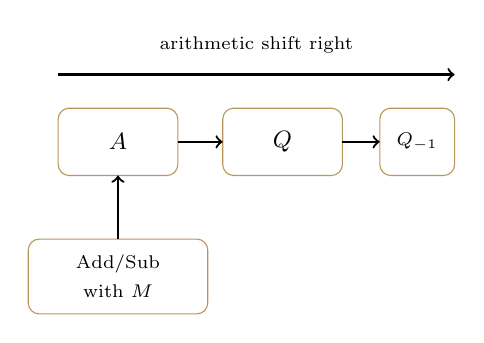
\begin{tikzpicture}[scale=0.95, transform shape,
      every node/.style={font=\small}]
    \node[draw=primary-gold, fill=white, rounded corners,
          minimum width=1.6cm, minimum height=0.9cm, align=center] (A) at (0,0) {$A$};
    \node[draw=primary-gold, fill=white, rounded corners,
          minimum width=1.6cm, minimum height=0.9cm, align=center] (Q) at (2.2,0) {$Q$};
    \node[draw=primary-gold, fill=white, rounded corners,
          minimum width=1.0cm, minimum height=0.9cm, align=center] (Qm1) at (4.0,0) {\scriptsize $Q_{-1}$};
    \draw[->, thick] (0.8,0) -- (1.4,0);
    \draw[->, thick] (3.0,0) -- (3.5,0);
    \draw[->, thick] (-0.8,0.9) -- (4.5,0.9);
    \node[font=\scriptsize] at (1.85,1.3) {arithmetic shift right};
    \node[draw=primary-gold, fill=white, rounded corners,
          minimum width=2.4cm, minimum height=1.0cm, align=center] (AS) at (0,-1.8) {\scriptsize Add/Sub\\\scriptsize with $M$};
    \draw[->, thick] (0,-1.3) -- (0,-0.45);
  \end{tikzpicture}
  \caption{Booth's algorithm datapath: the $A/Q/Q_{-1}$ shift register with an Add/Sub-with-$M$ block feeding $A$.}
  \label{fig:booth}
\end{figure}

\begin{example}[$13 \times (-6)$ by Booth's algorithm]
5-bit two's complement, $M=13=01101$, $Q=-6=11010$:
\begin{center}
\small
\begin{tabular}{@{}cccl@{}}
\toprule
Cycle & $(Q_0,Q_{-1})$ & Operation & $A$ after shift \\
\midrule
1 & $(0,0)$ & shift only & $00000$ \\
2 & $(1,0)$ & $A\gets A-M$, shift & $11001$ \\
3 & $(0,1)$ & $A\gets A+M$, shift & $00011$ \\
4 & $(1,0)$ & $A\gets A-M$, shift & $11011$ \\
5 & $(1,1)$ & shift only & $11101$ \\
\bottomrule
\end{tabular}
\end{center}
$(A,Q) = 1110110010_2 = -78$. \good{$13\times(-6)=-78$. Correct.}
\end{example}

\begin{teachingaside}
Students will assume the saving is in \emph{cycles} --- it is not; Booth's always runs $n$ cycles, same as shift-and-add. The saving is in \emph{arithmetic operations}: a run of consecutive 1s in $Q$ collapses to one subtract (at the run's start) and one add (just past its end). Push this with the worst case: alternating bits ($0101\dots$) give an add/sub \emph{every} cycle, so Booth's does no better than shift-and-add there --- it is never worse, and strictly better whenever $Q$ has a run of two or more equal bits.
\end{teachingaside}

\textbf{A question worth asking live}: ``Booth's always runs $n$ cycles --- so where exactly is the saving, and is there a multiplier pattern where Booth's does no better than plain shift-and-add?'' (Answer above --- pose it before revealing the alternating-bits case.)

\begin{example}[Extra: $(-9) \times 5$ by Booth's algorithm]
A second, independently verified instance --- 5-bit two's complement, $M=-9=10111$, $Q=5=00101$, $Q_{-1}=0$, $A=00000$:
\begin{center}
\small
\begin{tabular}{@{}cccl@{}}
\toprule
Cycle & $(Q_0,Q_{-1})$ & Operation & $A$ after shift \\
\midrule
1 & $(1,0)$ & $A\gets A-M$, shift & $00100$ \\
2 & $(0,1)$ & $A\gets A+M$, shift & $11101$ \\
3 & $(1,0)$ & $A\gets A-M$, shift & $00011$ \\
4 & $(0,1)$ & $A\gets A+M$, shift & $11101$ \\
5 & $(0,0)$ & shift only & $11110$ \\
\bottomrule
\end{tabular}
\end{center}
Final $Q=10011$, so $(A,Q)=1111010011_2$. Two's complement decode: invert $\to 0000101100$, $+1 \to 0000101101 = 45$, so the value is $-45$. \good{$(-9)\times 5 = -45$. Correct.} Have this one ready on a slip of paper --- it exercises a negative multiplicand, which the thread example does not.
\end{example}

\section{Division Algorithms}

Open with long division by hand: bring down a digit, subtract the divisor as many times as it fits, record the count, repeat. In binary ``as many times as it fits'' collapses to \emph{once or zero times per bit}, so division becomes shift, subtract, and a one-bit decision. Frame the two hardware strategies as differing only in what happens when the subtraction goes negative.

\begin{definitionbox}{Restoring Division}
Registers $A$ (remainder, init 0), $Q$ (dividend $\to$ quotient), $M$ (divisor). Repeat $n$ times: (1) shift $(A,Q)$ left 1 bit; (2) $A \gets A-M$; (3) if $A<0$, \key{restore} $A \gets A+M$ and set $Q_0=0$, else set $Q_0=1$. Every cycle does a subtract, and on average half the time an extra restoring add --- up to 2 arithmetic operations per cycle. (P\&H, Sec.~3.4, p.197; Hamacher Ch.~6, Sec.~6.6, p.390-392) \cite{PattersonHennessy2017_computer_organization_design,Hamacher2002_computer_organization}
\end{definitionbox}

\begin{definitionbox}{Non-Restoring Division}
Same registers. Repeat $n$ times: (1) shift $(A,Q)$ left 1 bit; (2) if $A\ge0$, $A\gets A-M$, else $A\gets A+M$; (3) if $A\ge0$, set $Q_0=1$, else $Q_0=0$. After $n$ cycles, if $A<0$ a single final correction $A\gets A+M$ recovers the true remainder ($Q$ is already correct). Exactly \emph{one} arithmetic operation per cycle, always --- no restore step.
\end{definitionbox}

\textbf{How to present it:} draw the two flowcharts (Figure~\ref{fig:division}) as two separate columns, left then right, with the dashed divider drawn last so it visually reads as ``two independent procedures,'' not one diagram with a branch. Before revealing the Non-Restoring column, ask the class to predict box 2 given only the rule ``never restore, carry the negative remainder forward.''

\begin{figure}[h]
  \centering
  % Diagram: two independent 3-box flowcharts, Restoring (left, x=-2.6) and
  % Non-Restoring (right, x=2.6), 2.0 units apart edge-to-edge, dashed
  % divider at x=0 in the empty gap. Copied verbatim from
  % Slides/CS401/02-number-systems-arithmetic.tex ("Restoring vs.
  % Non-Restoring, Side by Side" frame) -- P7 clearance re-audited
  % 2026-08-10: header labels at y=3.1 clear box tops at y=2.6 by 0.5cm
  % (P7c); connecting arrows sit only in the inter-box gaps, crossing no
  % box (P7a); no on-line labels (P7b); no plotted curves (P7d n/a).
  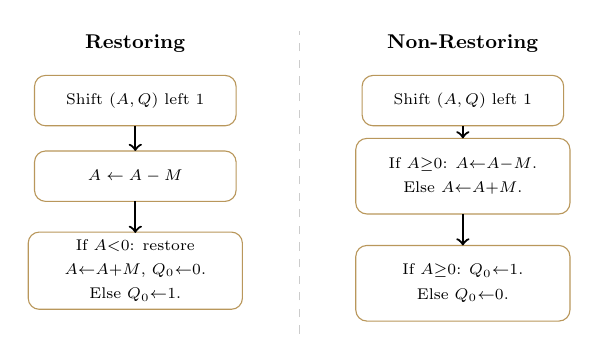
\begin{tikzpicture}[scale=0.8, transform shape,
      every node/.style={font=\small}]
    \draw[dashed, gray!40] (0,-1.5) -- (0,3.3);
    \node[font=\small, align=center] at (-2.6,3.1) {\textbf{Restoring}};
    \node[draw=primary-gold, fill=white, rounded corners,
          minimum width=3.2cm, minimum height=0.8cm, align=center] (R1) at (-2.6,2.2) {\scriptsize Shift $(A,Q)$ left 1};
    \node[draw=primary-gold, fill=white, rounded corners,
          minimum width=3.2cm, minimum height=0.8cm, align=center] (R2) at (-2.6,1.0) {\scriptsize $A \gets A - M$};
    \node[draw=primary-gold, fill=white, rounded corners,
          minimum width=3.4cm, minimum height=1.2cm, align=center] (R3) at (-2.6,-0.5) {\scriptsize If $A{<}0$: restore\\\scriptsize $A{\gets}A{+}M$, $Q_0{\gets}0$.\\\scriptsize Else $Q_0{\gets}1$.};
    \draw[->, thick] (-2.6,1.8) -- (-2.6,1.4);
    \draw[->, thick] (-2.6,0.6) -- (-2.6,0.1);
    \node[font=\small, align=center] at (2.6,3.1) {\textbf{Non-Restoring}};
    \node[draw=primary-gold, fill=white, rounded corners,
          minimum width=3.2cm, minimum height=0.8cm, align=center] (N1) at (2.6,2.2) {\scriptsize Shift $(A,Q)$ left 1};
    \node[draw=primary-gold, fill=white, rounded corners,
          minimum width=3.4cm, minimum height=1.2cm, align=center] (N2) at (2.6,1.0) {\scriptsize If $A{\ge}0$: $A{\gets}A{-}M$.\\\scriptsize Else $A{\gets}A{+}M$.};
    \node[draw=primary-gold, fill=white, rounded corners,
          minimum width=3.4cm, minimum height=1.2cm, align=center] (N3) at (2.6,-0.7) {\scriptsize If $A{\ge}0$: $Q_0{\gets}1$.\\\scriptsize Else $Q_0{\gets}0$.};
    \draw[->, thick] (2.6,1.8) -- (2.6,1.6);
    \draw[->, thick] (2.6,0.4) -- (2.6,-0.1);
  \end{tikzpicture}
  \caption{Restoring vs.\ non-restoring division, side by side. Both repeat $n$ times; restoring can spend 2 arithmetic ops/cycle, non-restoring always spends exactly 1 (plus one final correction).}
  \label{fig:division}
\end{figure}

\begin{example}[$13 \div 3$, both algorithms]
4-bit unsigned, $Q=13=1101$ (dividend), $M=3=0011$ (divisor). Both run 4 cycles and must agree: quotient $Q=4=0100$, remainder $A=1=0001$ ($13=4\times3+1$). \good{Both algorithms converge on the same result; non-restoring gets there with fewer arithmetic operations.} Full per-cycle traces for both algorithms on this pair are in the Lecture Notes (Sec.~2.7, Example).
\end{example}

\begin{teachingaside}
The recurring misconception here is that non-restoring division feels ``incomplete'' because it skips the restore step --- students expect the intermediate remainder to always be correct. It is not, and that is fine: the negative partial remainder is carried forward and \emph{compensated} by the next cycle's operation choice, with only the \emph{final} value needing at most one correction. Emphasize that both algorithms compute the identical quotient and remainder; the difference is purely how much arithmetic work gets done to get there.
\end{teachingaside}

\textbf{A question worth asking live}: ``restoring division does a subtract every cycle, plus a restoring add whenever $A<0$; non-restoring does exactly one add-or-subtract every cycle. Which does more total arithmetic operations, and why can non-restoring never do more?'' (Restoring: up to 2 ops/cycle. Non-restoring: exactly 1 op/cycle plus at most one final correction --- never more than restoring, often fewer.)

\begin{example}[Extra: $11 \div 3$ by restoring division]
A second, independently verified instance --- 4-bit unsigned, $Q=11=1011$ (dividend), $M=3=0011$ (divisor), $A=0000$:
\begin{center}
\small
\begin{tabular}{@{}clcll@{}}
\toprule
Cycle & Shift $(A,Q)$ & $A\gets A-M$ & Decision & $A,Q$ after \\
\midrule
1 & $A{=}0001,Q{=}0110$ & $A=1110$ (neg.) & restore, $Q_0{=}0$ & $A{=}0001,\,Q{=}0110$ \\
2 & $A{=}0010,Q{=}1100$ & $A=1111$ (neg.) & restore, $Q_0{=}0$ & $A{=}0010,\,Q{=}1100$ \\
3 & $A{=}0101,Q{=}1000$ & $A=0010$ ($\ge0$) & keep, $Q_0{=}1$ & $A{=}0010,\,Q{=}1001$ \\
4 & $A{=}0101,Q{=}0010$ & $A=0010$ ($\ge0$) & keep, $Q_0{=}1$ & $A{=}0010,\,Q{=}0011$ \\
\bottomrule
\end{tabular}
\end{center}
$Q=0011=3$ (quotient), $A=0010=2$ (remainder). \good{$11 = 3\times3+2$. Correct.} Non-restoring division on the same pair converges to the identical $Q=3,\,A=2$ with fewer arithmetic operations --- worth tracing on the board only if time allows; the point (same answer, less work) is already made.
\end{example}

\section{Synthesis and Summary}

Close the thread: $+7 + (-3)$ used every tool from the first sections --- two's complement representation, addition without subtraction hardware, the ripple-carry adder, the discarded carry-out, and the sign check for overflow. The result $0100 = +4$ is the same number a human computes, but now it is the output of a specific circuit. The \emph{same} adder, driven by different control logic, then extended the thread to multiplication (Booth's algorithm: examine $(Q_0,Q_{-1})$, add/subtract/no-op, then arithmetic-shift-right --- computing $13\times(-6)=-78$) and division (shift, subtract, one-bit decision --- restoring and non-restoring both computing $13\div3=4$ remainder $1$, differing only in efficiency). No new arithmetic hardware was needed beyond the adder built earlier in the lecture.

Set up Week 3: fixed point handles fractions but with fixed range/precision; real numbers span $10^{-300}$ to $10^{300}$; Week 3 builds IEEE\,754 floating point --- sign, exponent, mantissa --- trading a little precision for a huge range.

\textbf{Summary --- quick reference:} \emph{Number systems:} value $= \sum d_i r^i$; convert by repeated division; hex/octal group bits. \emph{Two's complement:} $-2^{n-1} \le x \le 2^{n-1}-1$; negate by flip + 1; addition needs no special subtraction hardware. \emph{Overflow:} carry-out $\neq$ overflow; wrong result sign is the test. \emph{Fixed point:} an agreed binary point; simple but limited range and precision. \emph{Adder:} HA/FA equations; ripple-carry chain; $A-B = A+(-B)$. \emph{Booth's algorithm:} $(Q_0,Q_{-1})$ recoding --- $(0,1)$ adds, $(1,0)$ subtracts, $(0,0)$/$(1,1)$ shift only; never worse than shift-and-add. \emph{Division:} restoring subtracts then conditionally restores (up to 2 ops/cycle); non-restoring always does exactly 1 op/cycle.

\bibliographystyle{plain}
\bibliography{../../Bibliography_base}

\end{document}
